\chapter{Vyhledávací stromy}

V~této kapitole zavedeme formální definici binárního vyhledávacího stromu a
pojednáme o~jeho výhodách oproti jiným způsobům uložení dat. Dále přiblížíme
(staticky) optimální strom. Pro dynamické stromy připomeneme některé běžné
vyvažovací strategie a také představíme jiné, novější přístupy, například třídu
rankově vyvážených stromů a jejich speciální případ Weak AVL strom. Potom
představíme několik mezí optimality -- vlastností, které musí mít optimální
binární vyhledávací strom. Nakonec se podíváme na tango stromy a multisplay
stromy a dokážeme, že tyto meze splňují (nebo, v~případě tango stromu, že je
téměř splňují).

\section{Binární vyhledávací stromy}
\def\U{\mathcal U}
\def\o{\mathcal O}
\let\op\operatorname

Častým úkolem datové struktury je udržovat informaci o~množině prvků. Formálně
mějme univerzum $\mathcal U$, lineární uspořádání na tomto univerzu $\leq$ a
konečnou podmnožinu tohoto univerza $M$. Budeme chtít vybudovat datovou strukturu, která dokáže
o~každém prvku $\mathcal U$ říct, zda náleží množině $M$. Po takových
strukturách často požadujeme nějaké z~následujících operací:

\begin{itemize}
\item $\ope{Build}(M)$: vystavět novou strukturu nad množinou $M$,
\item $\ope{Find}(x)$: pro prvek $x \in \U$ rozhodnout, zda $x\in M$,
\item $\ope{Insert}(x)$: přidat prvek $x \in \U$ do množiny $M$,
\item $\ope{Delete}(x)$: odstranit prvek $x\in M$ z~$M$,
\item $\ope{Enumerate}$: vyjmenovat všechny prvky $M$,
\item $\ope{Succ}(x)$, respektive $\ope{Pred}(x)$: pro daný prvek $x\in \U $ najít nejbližší (ostře) větší, respektive menší prvek $M$,
\item $\ope{RangeQuery}(x,y)$: pro dané dva prvky $x,y\in\U$ takové, že $x<y$, spočítat nebo vyjmenovat všechny prvky $z\in M$ takové, že $x \leq z \leq y$.
\end{itemize}

Volba struktury vždy závisí na tom, které z~těchto
operací potřebujeme v~naší konkrétní aplikaci podporovat. Pokud nám například
stačí umět prvky vyjmenovat, postačí nám obyčejné pole. Pokud chceme umět
vyhledávat, přidávat i mazat v~průměru v~konstantním čase, je nejlepší volbou nějaká
varianta hashovací tabulky. Zejména \ope{Succ}, \ope{Pred} a \ope{RangeQuery} ale hashovací
tabulka umí pouze v~čase $\Theta(|M|)$. Pokud tedy tento typ dotazů potřebujeme
struktuře pokládat, můžeme využít některou ze stromových datových struktur,
které v~této práci popíšeme.

\begin{definice}

\emph{Binární vyhledávací strom} je struktura, které může být buď prázdná, nebo
může obsahovat vrchol, který nazveme \emph{kořen}. Kořen má dva ukazatele,
které opět ukazují na (ne nutně neprázdné) binární vyhledávací stromy. Kořenům těchto stromů budeme říkat \emph{pravý} a \emph{levý syn} kořene. Pokud je vrchol $v$ synem vrcholu $u$, řekneme, že vrchol $u$ je rodičem vrcholu $v$. Na každý vrchol stromu krom kořene musí ukazovat právě jeden ukazatel z~rodiče. 

Pro vrchol $v$ nazveme
\emph{podstromem vrcholu $v$} množinu vrcholů, do nichž se dá dostat z~vrcholu
$v$ libovolnou\footnote{Posloupnost může být i prázdná.} posloupností kroků 
\uv{přejdi do pravého syna} a \uv{přejdi do levého syna}. Podstromu pravého, respektive levého syna vrcholu $v$ budeme také říkat \emph{levý} a \emph{pravý podstrom} vrcholu $v$

V~každém vrcholu bude pak právě jedna \emph{hodnota} nebo také \emph{klíč}, a navíc bude pro každý vrchol~$v$ platit, že hodnoty ve všech vrcholech v~levém podstromu $v$ jsou ostře menší než hodnota ve $v$ a hodnoty v~pravém podstromu naopak ostře větší.
\end{definice}

Při práci se stromem budeme předpokládat, že následující kroky umíme v~konstantním čase:
\begin{itemize}
\item Nalezni kořen,
\item přejdi do pravého, případně levého syna aktuálního vrcholu,
\item přejdi do rodiče aktuálního vrcholu,
\item přečti či zapiš hodnotu v~aktuálním vrcholu,
\item pokud aktuální vrchol nemá pravého či levého syna, vytvoř na jeho místě nový vrchol s~danou hodnotou.
\end{itemize}
Vyhledávání hodnoty $x$ ve stromu pak můžeme provést podle následujícího algoritmu:
\begin{enumerate}
\item Nalezni kořen.
\item Podívej se, zda je hodnota $x$ rovna hodnotě v~aktuálním vrcholu, a pokud ano, nahlas nález.
\item Je-li hodnota $x$ větší než hodnota v~aktuálním vrcholu, podívej se, zda existuje pravý syn aktuálního vrcholu. Pokud ano, přejdi do něj a vrať se ke 2. kroku algoritmu, jinak ohlas, že  $x$ ve stromu není.
\item Je-li hodnota $x$ menší než hodnota v~aktuálním vrcholu, podívej se, zda existuje levý syn aktuálního vrcholu. Pokud ano, přejdi do něj a vrať se ke 2. kroku algoritmu, jinak ohlas, že  $x$ ve stromu není.
\end{enumerate}

Podobným algoritmem budeme prvky přidávat, pouze místo nahlášení neexistence $x$ na místě chybějícího syna založíme nový vrchol. Mazání prvku provedeme následovně:

\begin{itemize}
\item Je-li vrchol obsahující mazaný prvek list, prostě ho smaž.
\item Má-li vrchol obsahující mazaný prvek právě jednoho syna, prvek smaž a jeho syna připoj pod rodiče mazaného prvku na místo mazaného prvku.
\item Má-li vrchol obsahující mazaný prvek dva syny, najdi ve stromu nejblížší větší prvek, jeho
hodnotu zapiš na místo odstraňovaného prvku a odstraň vrchol, v~němž byl uložen tento nejbližší větší
prvek. Tomuto vrcholu nutně chybí přinejmenším levý syn (kdyby existoval, hodnota
v~něm by byla menší než hodnota jeho rodiče, ale větší než hodnota odstraňovaného
vrcholu -- jeho rodič by tedy nemohl být nejbližší větší).  
\end{itemize} 

\section{Statická optimalita}\label{sec:staticoptimality}

Podívejme se na životní cyklus binárního vyhledávacího stromu. Takový strom
nejprve vybudujeme s~(ne nutně neprázdnou) počáteční množinou klíčů
a potom na něm vykonáme nějakou posloupnost operací. My se prozatím omezíme
pouze na případ, kdy strom vybudujeme nad neprázdnou množinou klíčů a jediná
operace, kterou budeme vykonávat, bude operace vyhledání. Navíc budeme
požadovat, aby se všechny klíče, které ve stromu hledáme, skutečně ve stromu nacházely.
Potom je posloupnost operací jednoznačně dána pouze hodnotami, na které se
dotazujeme (a jejich pořadím; hodnoty nemusí být různé). Posloupnost těchto
hodnot budeme nazývat \emph{přístupová posloupnost}, budeme ji značit $S$ a
její délku budeme značit $m$.

Přirozená otázka zní, jak vypadá binární vyhledávací strom, který pro danou
posloupnost přístupů vykoná nejméně kroků. V~plné obecnosti budeme tuto otázku řešit v~pozdějších částech této kapitoly. Pro tuto sekci se omezíme na statické
stromy. To znamená stromy, jejichž strukturu (tedy v jejich vrcholech uložené
ukazatele) po vybudování již mebudeme měnit. Na druhou stranu budeme
předpokládat, že přístupovou posloupnost, nebo alespoň četnost jednotlivých
prvků v~ní, předem známe. V~tomto modelu se počet kroků přesně rovná počtu
navštívených vrcholů (včetně násobnosti).

Problém konstrukce optimálního stromu v~tomto modelu vyřešil dynamickým
programováním \citet{staticoptimality}. Myšlenku jeho algoritmu zde představíme.

Mějme množinu klíčů, pro jednoduchost $[n]$ (tedy
množinu přirozených čísel od 1 do $n$ včetně), a pole vah $w$. 
Naším cílem bude najít strom nad množinou klíčů $[n]$ s co nejnižší celkovou vahou, kde váha stromu je $$\sum_{i\in [n]}w_i\cdot (\text{hloubka vrcholu obsahujícího $i$}).$$ 

Váha klíče
$i$ $w[i]$ může být buď pravděpodobnost, že daný přístup bude mít za
cíl klíč~$i$, nebo počet výskytů kíče~$i$ v~přístupové
posloupnosti. V~prvním případě dostaneme jako váhu výsledného stromu střední
hodnotu počtu navštívených vrcholů při přístupu, v~druhém případě součet počtů navštívených vrcholů přes
celou přístupovou posloupnost.

Algoritmus je založený na myšlence, že podstrom libovolného vrcholu
v~optimálním stromu je sám o~sobě optimálním stromem nad příslušnými prvky. Proto
stačí pro všechny možné volby kořene rekurzivně spočítat optimální strom pro
prvky menší než kořen a větší než kořen, a z~takto spočítaných stromů vybrat
ten s~nejmenší váhou. Protože přímočará implementace tohoto postupu by běžela
v~exponenciálním čase, budeme si váhy (a případně kořeny) dílčích optimálních
stromů ukládat. Tímto postupem postavíme optimální strom
v~čase $\Theta(n^3)$. Algoritmus lze však upravit tak, aby měl kvadratickou časovou složitost.



\section{Vyvažované stromy}

Co když však potřebujeme umět do struktury i vkládat? Můžeme pokračovat naivně
podle algoritmu uvedeného výše v~této kapitole. \citet{sortingsearching}
ukázal, že pokud budeme prvky do stromu vkládat v~náhodném pořadí,\footnote{Bez
újmy na obecnosti předpokládáme, že do struktury postupně vložíme všechny prvky
z~množiny $[n]$ pro vhodně zvolené $n$. Potom náhodné pořadí znamená pořadí
určené rovnoměrně náhodně zvolenou permutací na~množině $[n]$.} s~vysokou
pravděpodobností dostaneme strom, v~němž bude průměrná hloubka vrcholu $2 \ln n$.
\citet{Robson} dále ukázal, že pokud $H(n)$ je střední hodnota hloubky nejhlubšího 
vrcholu ve stromu o~$n$ vrcholech vytvořeného vložením hodnot v náhodném pořadí, pak $$\lim_{m\rightarrow
\infty}\frac{H(n)}{\ln(n)}\leq\alpha,$$ kde $\alpha$ je přibližně
$4.311\dots$, přesně se jedná o~největší kořen rovnice $$\alpha\cdot \ln
\frac{2\operatorname{e}}{\alpha} = 1.$$ \citet{devroye} později dokázal, že výše uvedená
nerovnost je ve skutečnosti rovnost.

V~praxi však často klíče potřebujeme vkládat i v~pořadí, které není náhodné,
ale obsahuje nějakou pravidelnost. Například pokud bychom do (na počátku prázdného)
nevyvažovaného binárního stromu vložili čísla z~množiny $[n]$ vzestupně, strom
zdegeneruje v~jednu jedinou cestu, na níž bude nejhlubší vrchol v~hloubce $n$ a
průměrná hloubka vrcholu bude $(n+1)/2$. Takovýmto případům bychom se rádi
vyhnuli, proto prozkoumáme vyvažované stromy. Protože však všechny stromy,
které budeme zkoumat, budou vyvažované pomocí rotací hran, představíme nejprve,
co taková rotace hrany je, a to jak obrázkem \ref{obr:rotace}, tak formální definicí.


\begin{figure}[h!]
\begin{tabular}{cc}

\begin{subfigure}{0.45\textwidth}
  \centering
  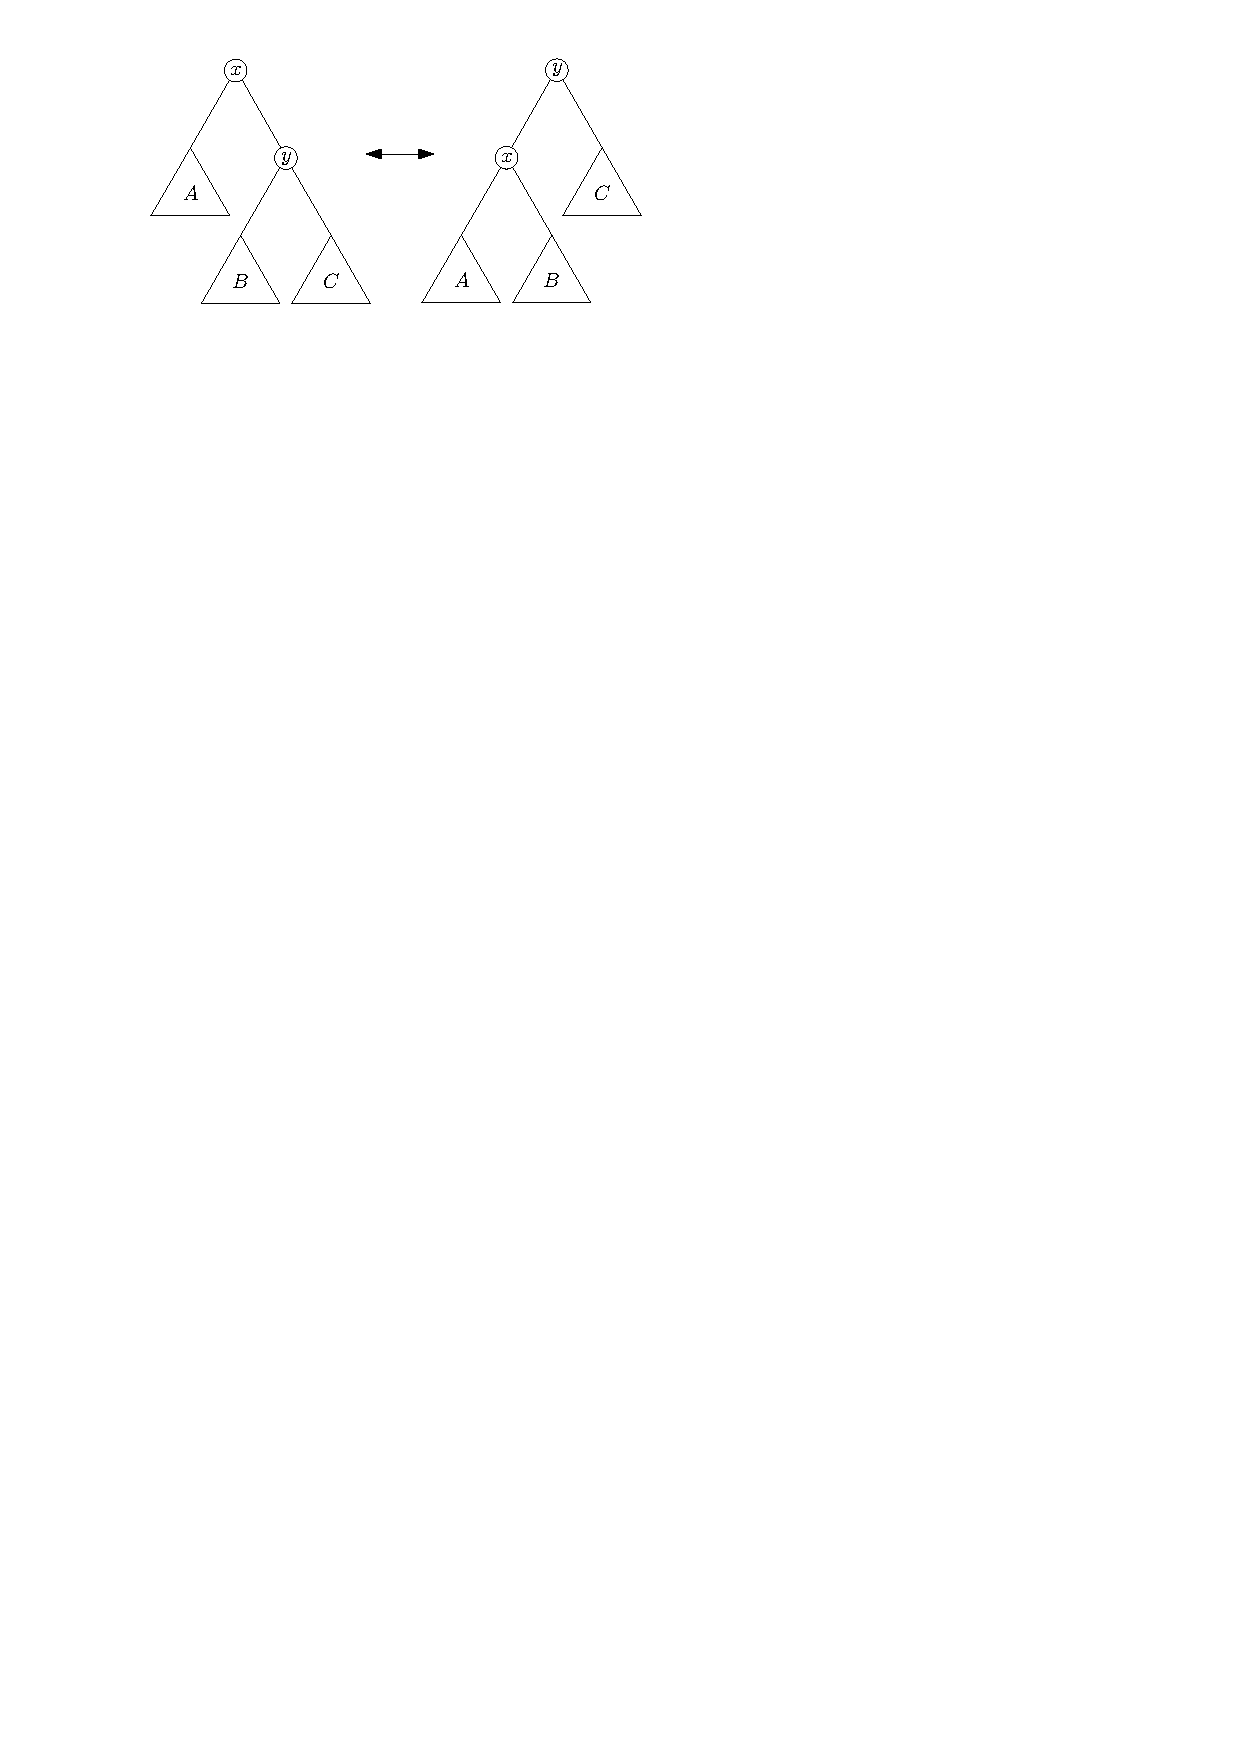
\includegraphics[width=.99\linewidth]{../img/single_rotation}
\end{subfigure}&

\begin{subfigure}{0.45\textwidth}
  \centering
  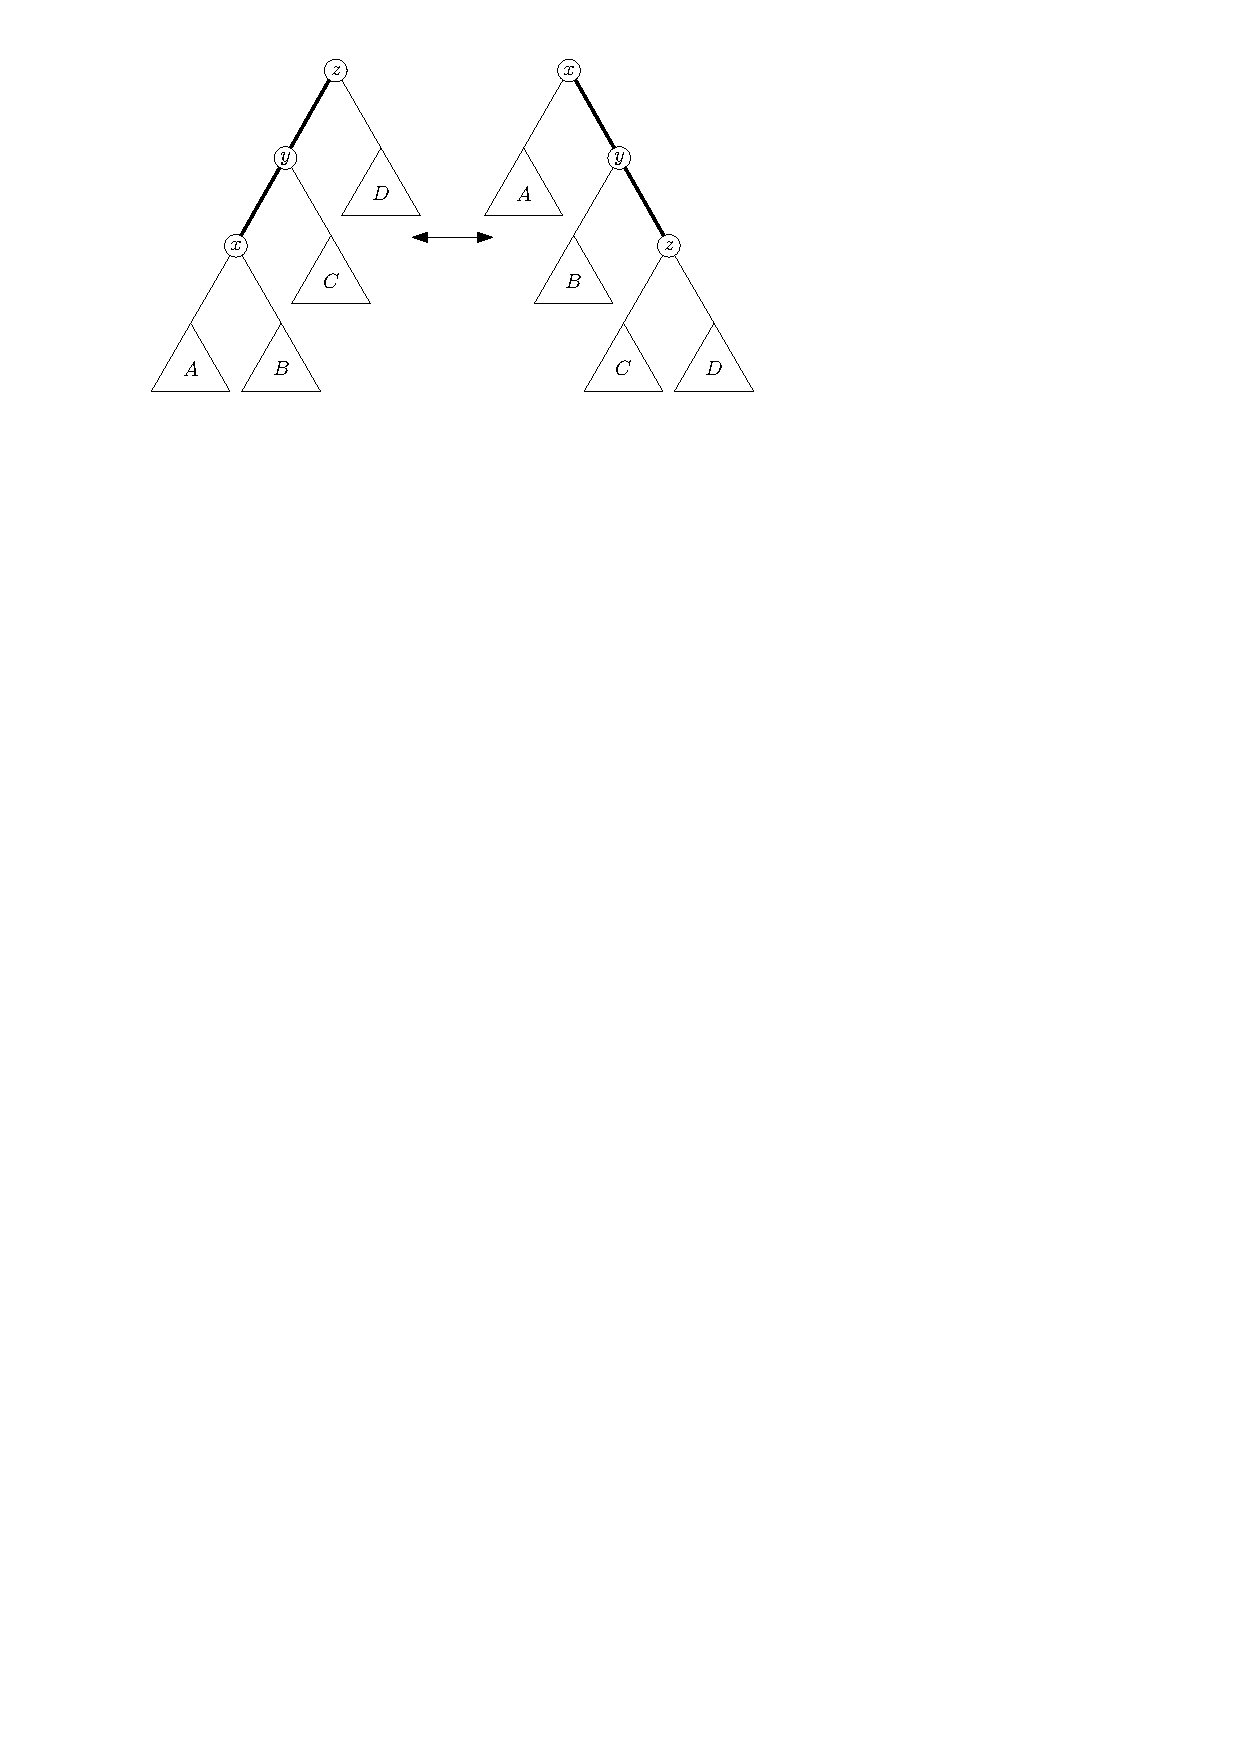
\includegraphics[width=.99\linewidth]{../img/zigzig_rotation}
\end{subfigure}\\

\noalign{\bigskip}
(a) Jednoduchá rotace hrany $xy$. 
&
(b) Zig-zig rotace.\\
\noalign{\bigskip}

\multicolumn{2}{c}{
\begin{subfigure}{0.9\textwidth}
  \centering
  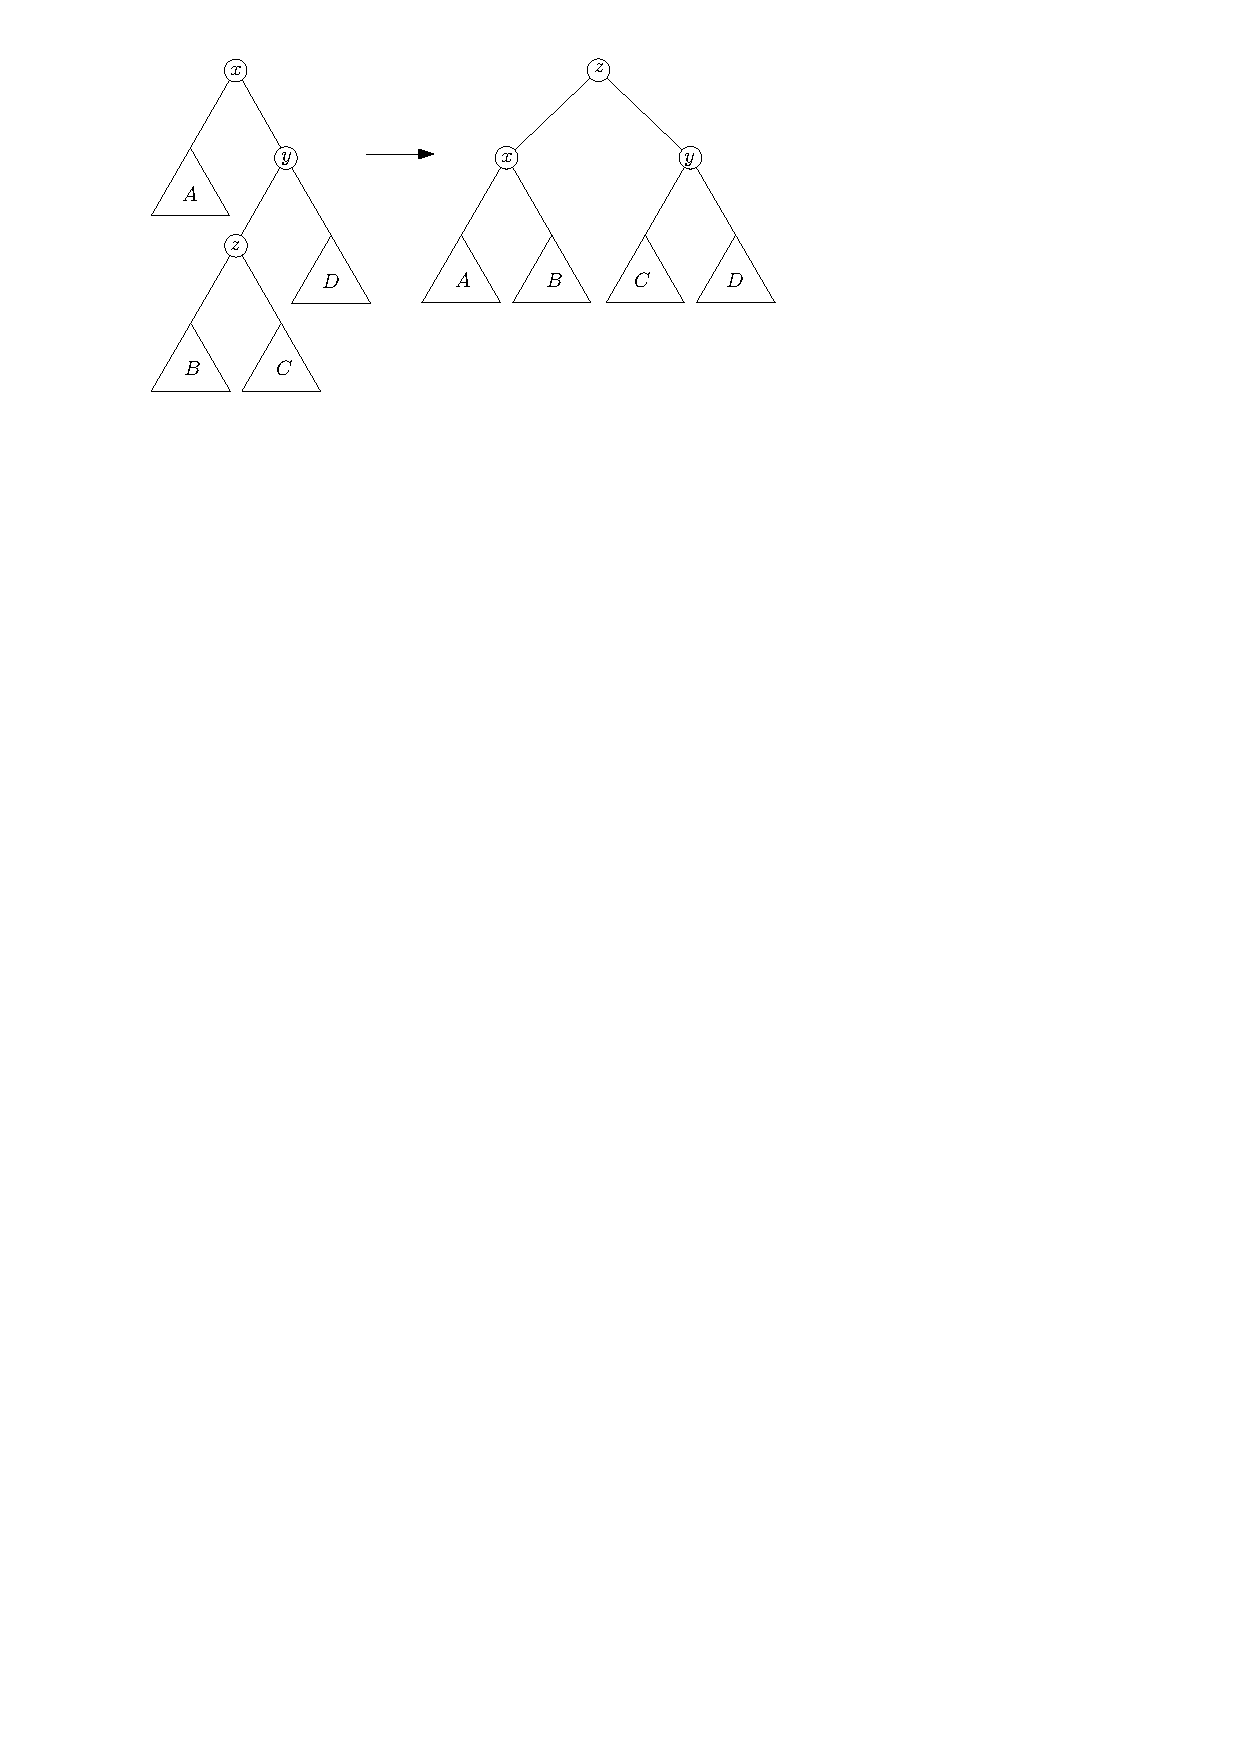
\includegraphics[width=.65\linewidth]{../img/zigzag_rotation}
\end{subfigure}}\\
\noalign{\bigskip}
\multicolumn{2}{c}{
  (c) Zig-zag rotace. Tato rotace jako jediná není symetrická.
}
\end{tabular} 
\caption{Jednoduchá, zig-zig a zig-zag rotace.} 

\label{obr:rotace} 
 
\end{figure}

\begin{definice}
Mějme vrchol binárního vyhledávacího stromu $x$ a jeho (bez újmy na obecnosti pravého) syna $y$. Dále
označme $p$ rodiče vrcholu $x$, $B$ a $C$ popořadě levý a pravý podstrom~$y$ a
$A$ levý podstrom $x$. Pak \emph{(jednoduchá) rotace hrany $xy$} je krok,
při němž nastavíme vrchol $y$ jako syna $p$ (na stejné straně, kde byl původně
vrchol $x$), vrchol $x$ jako levého syna $y$ a podstrom $B$ jako pravý podstrom~$u$. Podstromy $A$ a $C$ zůstanou připojené k~vrcholům $x$ a $y$ tak, jak byly.

Dále mějme vrchol $x$, jeho (bez újmy na obecnosti pravého) syna $y$ a syna
vrcholu~$y$, kterého označíme $z$. Potom, pokud $z$ je levý syn, můžeme
provést \emph{dvojitou rotaci hran $zy$ a $xz$ typu zig-zag}, která probíhá tak,
že nejprve zrotujeme hranu $zy$, a potom hranu $xz$. Pokud je $z$ pravý syn,
můžeme provést \emph{dvojitou rotaci hran $zy$ a $yx$ typu zig-zig}, která
probíhá tak, že nejprve zrotujeme hranu $yx$ a potom hranu $zy$.
\end{definice}

Rotace hrany se může jevit jako zvláštní operace. Téměř všechny vyvažovací
algoritmy (a úplně všechny, o~kterých zde budeme mluvit) ale využívají
k~vyvažování právě rotace, protože se jedná o~poměrně jednoduchou a překvapivě
silnou operaci, která mění strukturu stromu a přitom zachovává uspořádání.

Dvojité rotace typu zig-zig budeme používat později v~této kapitole. Pro teď
si vystačíme s~jednoduchými rotacemi a dvojitými rotacemi typu zig-zag,
proto budeme-li mluvit o~dvojitých rotacích, budeme tím mít na mysli právě typ
zig-zag.

\subsection{AVL stromy}

AVL strom poprvé představili \citet{AVL}. Jedná se o~typ vyvažovaného stromu.
V~AVL stromu platí, že hloubka pravého a levého podstromu každého vrcholu se liší
nejvýše o~jedna. To znamená, že pokud $D(n)$ označíme minimální počet vrcholů
ve stromu hloubky $n$, dostáváme, že $D(0)=0$, $D(1)=1$ a
$D(i)=1+D(i-1)+D(i-2)$ pro každé $i$ větší než jedna. Pokud vyřešíme tuto
rekurenci, zjistíme, že $D(i)=\log_\varphi(i) + \o(1)$, kde $$\varphi =\frac{1+\sqrt{5}}2 = 1.618\dots$$ je zlatý
řez.

V~každém vrcholu si budeme pamatovat navíc informaci o~vyvážení daného vrcholu.
Tato informace může nabývat tří možných hodnot -- příslušný vrchol může být buď
\emph{vyvážený} (oba jeho podstromy jsou stejně hluboké), nebo \emph{nakloněný
doprava} (jeho pravý podstrom je o~jedna hlubší než levý), nebo
\emph{nakloněný doleva}.\footnote{Vystačili bychom si i s~jediným bitem, který by udával, zda je podstrom daného vrcholu hlubší než podstrom jeho sourozence.}


\begin{figure}[h!]

\begin{subfigure}{0.9\textwidth}
  \centering
  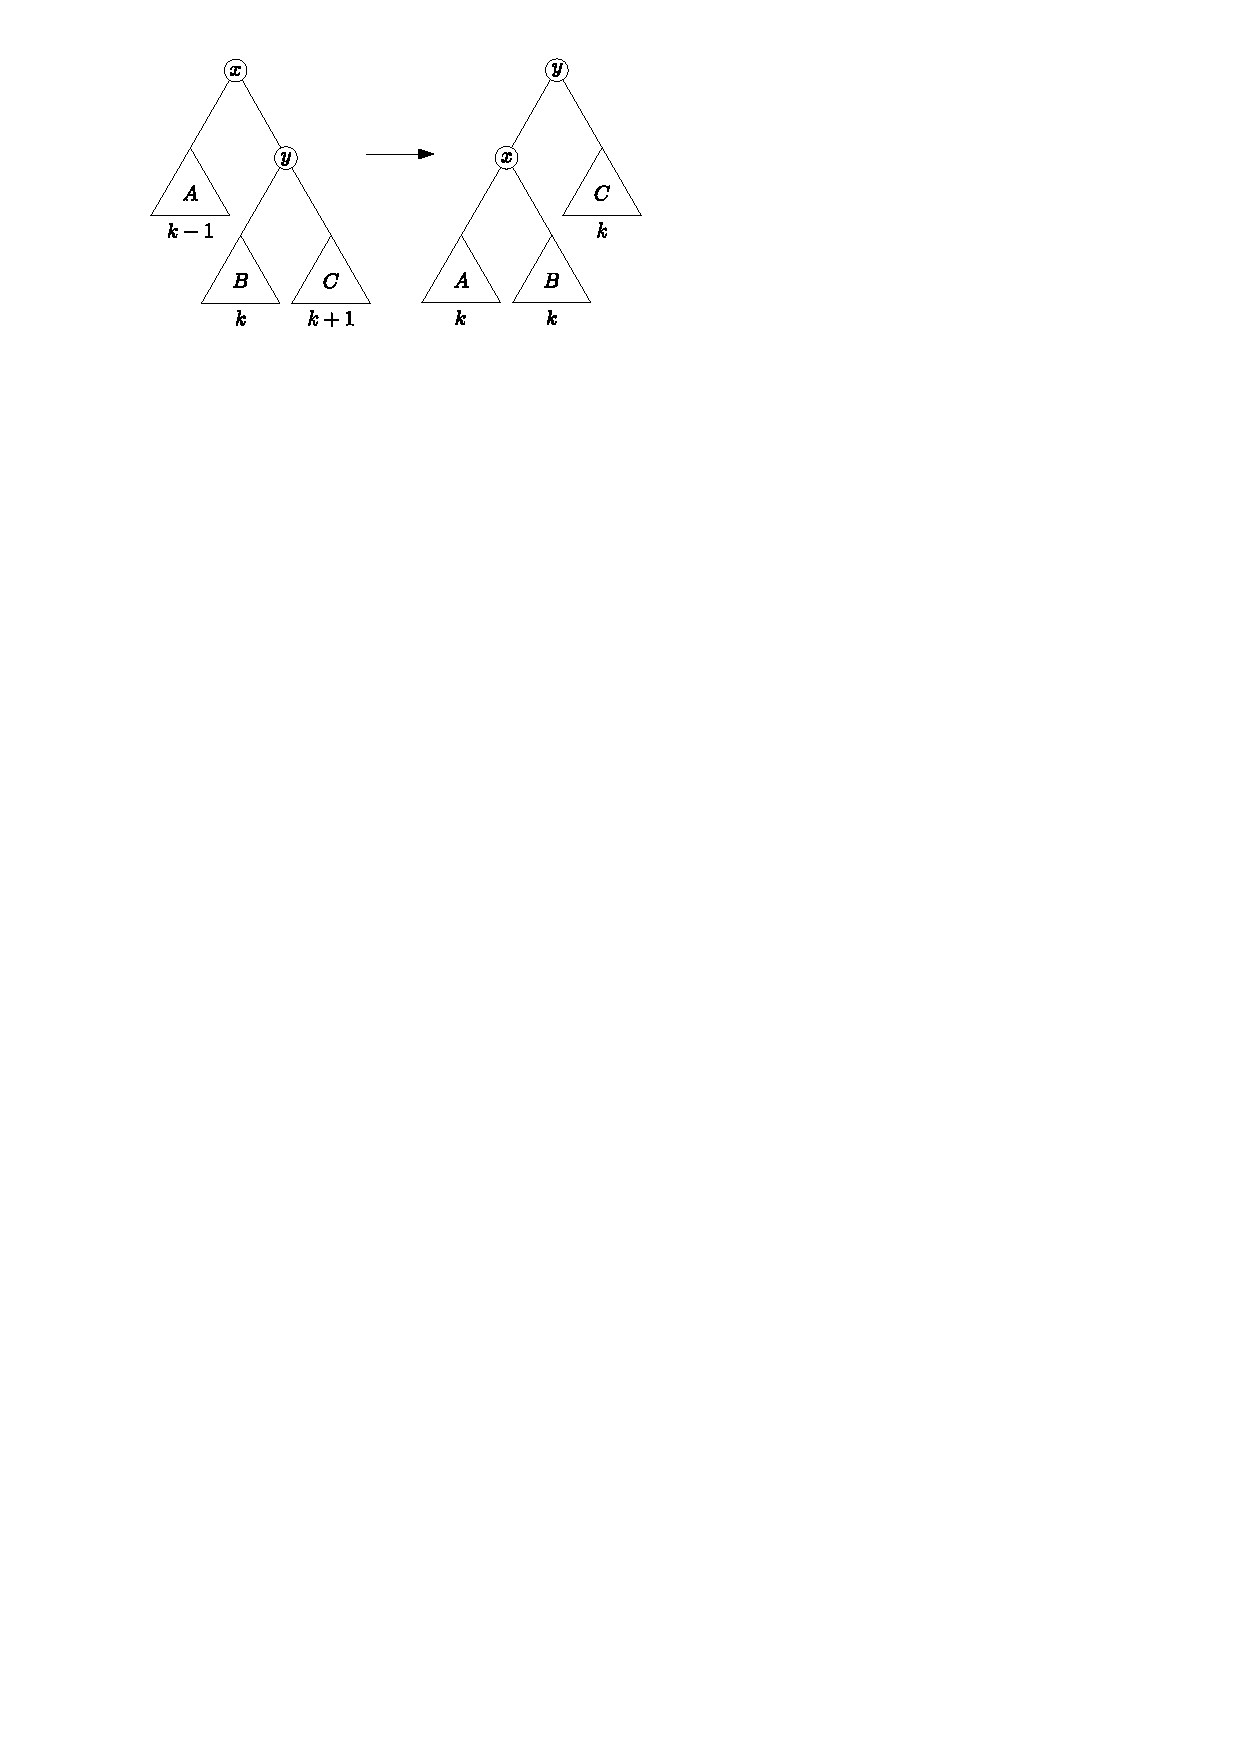
\includegraphics[width=.65\linewidth]{../img/single_rotation_avl}
\end{subfigure}
\vskip 1cm
\begin{subfigure}{0.9\textwidth}
  \centering
  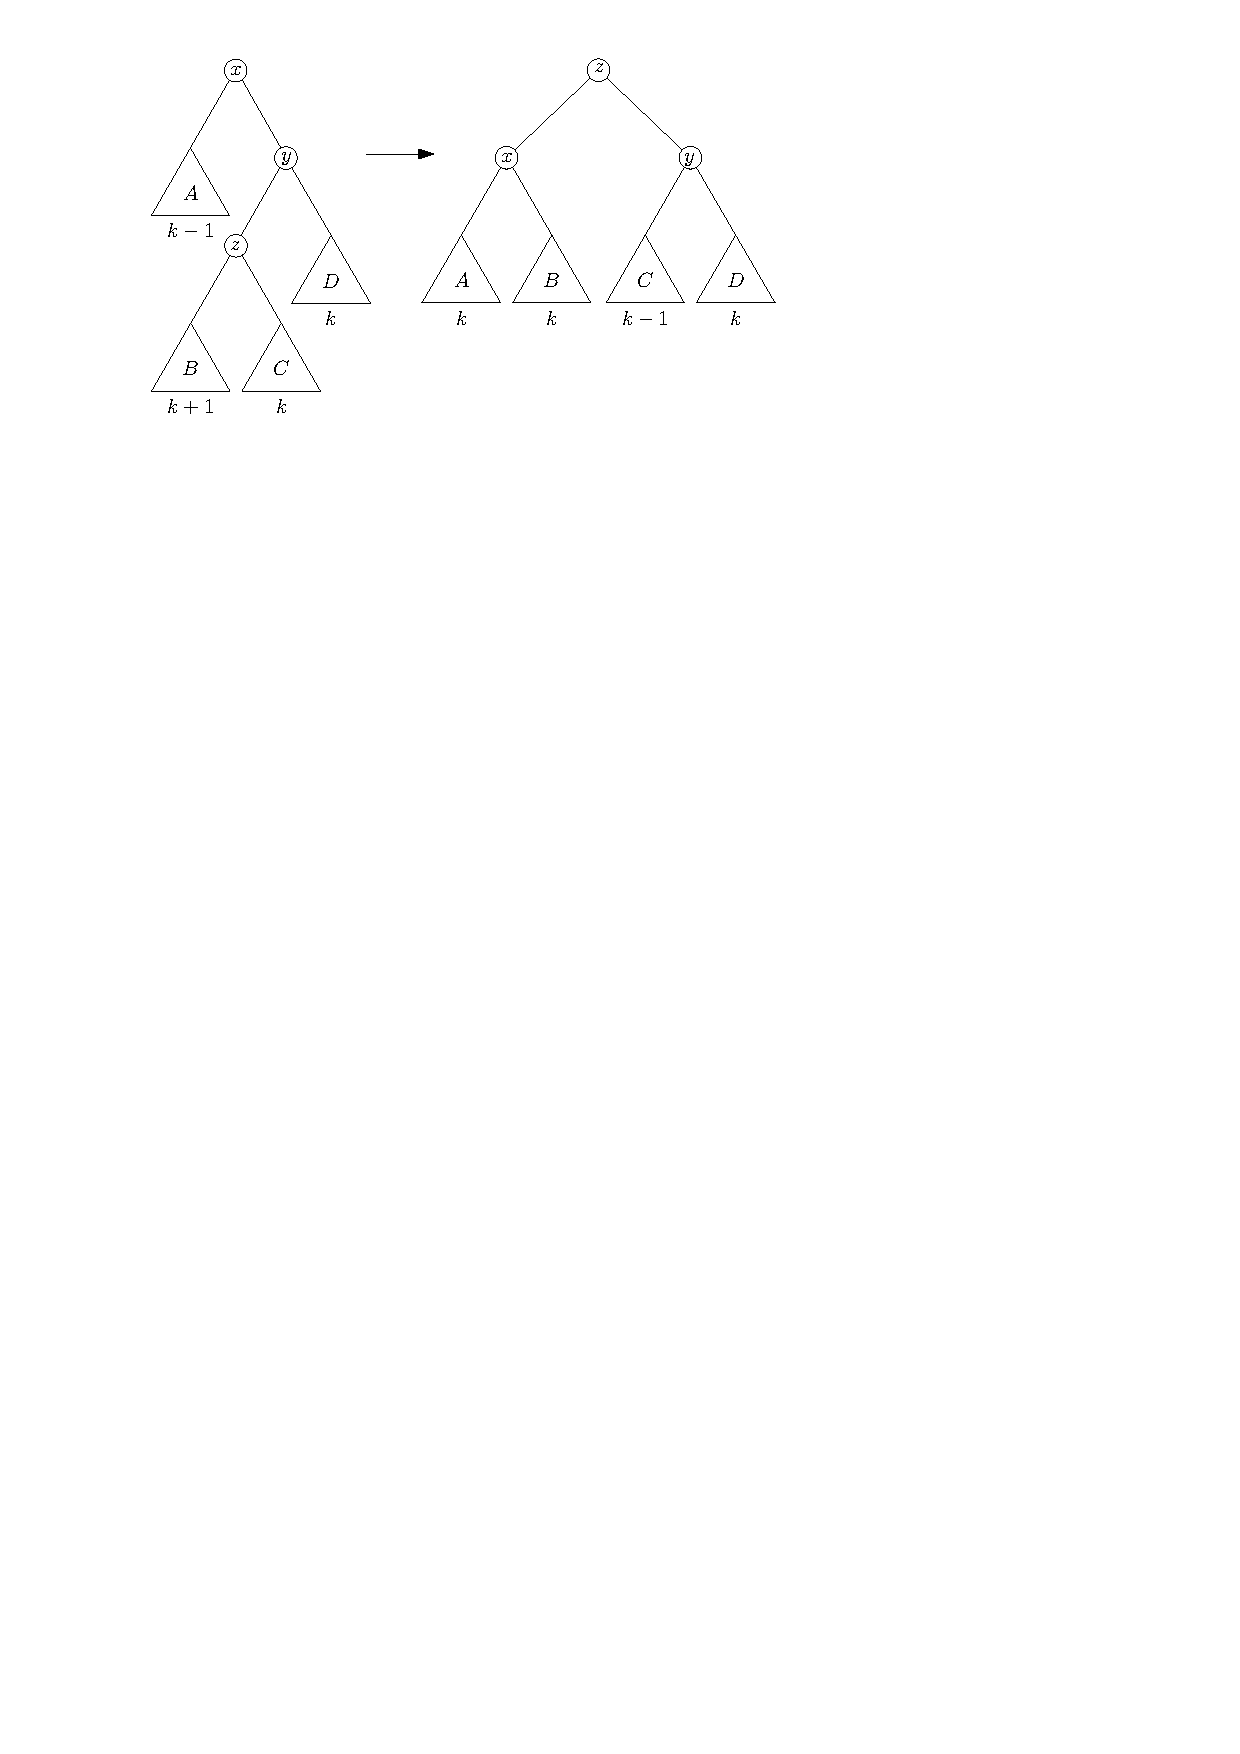
\includegraphics[width=.65\linewidth]{../img/zigzag_rotation_avl}
\end{subfigure}
\caption{Použití jednoduché a zig-zag rotace k~vyvážení AVL stromu.} 

\label{obr:rotace_avl} 
 
\end{figure}



Vyhledání prvku probíhá stejně, jako v~nevyvažovaném binárním vyhledávacím stromu. 
Vložení je ale trochu komplikovanější. Při připojení nového listu je potřeba
jeho rodiči změnit vyvážení. Byl-li vyvážený (tj. byl to list), nově bude
nakloněný za novým vrcholem. Byl-li nakloněný od nového vrcholu, bude nově
vyvážený. V~prvním případě navíc vzrostla celková hloubka podstromu tohoto
vrcholu, je tedy potřeba změnu vyvážení propagovat výše do stromu. Kromě
předchozích dvou případů  může při další propagaci nastat ještě jeden jiný,
totiž že byl vrchol už původně nakloněný směrem, ze kterého propagujeme. To
znamená, že po přidání nového vrcholu již neplatí invariant AVL stromu a musíme
provést buď jednoduchou, nebo dvojitou rotaci hrany, abychom situaci napravili.

Nechť $x$ je nejhlubším vrcholem ve stromu, který po vložení vrcholu $v$
nesplňuje AVL invariant. Hloubku jeho podstromu před vložením $v$ si označíme
$k$. Nechť byl bez újmy na obecnosti vložen vrchol do podstromu jeho pravého
syna~$y$. Pak je nutné rozebrat následující případy:

\begin{itemize}
\item Nový vrchol byl vložen do pravého podstromu vrcholu $y$ (první případ na
obrázku \ref{obr:rotace_avl}). Potom lze jednoznačně dopočítat hloubky
ostatních relevantních vrcholů (na obrázku pod podstromy; vždy počítáno vůči
kořenu nakreslené části stromu) na základě toho, že víme, že:
\begin{itemize}
\item Vrchol $x$ musí porušovat AVL
invariant, \item ostatní vrcholy ho musí splňovat, \item před vložením nového vrcholu
musely AVL invariant splňovat všechny vrcholy, \item hloubka podstromu $x$ musela
být $k$. 
\end{itemize}
Pak můžeme AVL invariant opravit jednoduchou rotací.  

\item Nový
vrchol byl vložen do levého podstromu $y$. Potom musíme provést
dvojitou rotaci. Jednu z~možných kombinací hloubek jednotlivých podstromů v~takovém případě zobrazuje
druhý případ na obrázku \ref{obr:rotace_avl}. Další možnost, kterou však není potřeba v~kódu
rozlišovat a vyřešíme ji úplně stejně, spočívá v~prohození hloubek podstromů
$B$ a $C$ z~tohoto obrázku.  
\end{itemize}

Provedením rotace však zařídíme, že se celý podstrom rotovaného vrcholu o~jedna
sníží. To znamená, že bude mít stejnou výšku jako před \ope{Insert}em a změnu tedy
není potřeba dále propagovat. Nabízí se otázka, když vyvažováním vždy
zajistíme, že se hloubka stromu nezmění, jak je možné, že do něj můžeme
postupně vložit libovolně mnoho vrcholů? Je to tím, že celková hloubka stromu
se může změnit právě při takových \ope{Insert}ech, které nezpůsobí žádnou
rotaci hrany.

Operaci \ope{Delete} zde podobně detailně probírat nebudeme, podotkneme ale, že na rozdíl od operace \ope{Insert} může být nutné až řádově logaritmicky mnoho rotací vůči vůči počtu vrcholů ve stromu (tj. lineárně mnoho vůči hloubce stromu). Kdybychom strom nejprve postavili posloupností operací \ope{Insert} a poté vymazali všechny vrcholy posloupností operací \ope{Delete}, mohli bychom ukázat, že provedeme amortizovaně konstantně mnoho rotací na operaci. Pokud však operace \ope{Insert} a \ope{Delete} nevhodně proložíme, může se stát, že budeme potřebovat až logaritmicky mnoho rotací na operaci.



\subsection{Červenočerné stromy}\label{sec:RB}

\citet{btrees} představili B-stromy. Těmi se zde nebudeme blíže zabývat, protože se nejedná o binární stromy. Z jejich speciálního případu (2,4) stromů ale \citet{redblack} odvodili červenočerné stromy, které si nyní popíšeme. K~tomu se nám bude hodit alternativní pohled na binární stromy.
Představíme si, že na každé místo ve stromu, kde některému vrcholu chybí pravý nebo levý syn, přidáme jeden list.
Tím dostaneme strom, v~němž bude každý vrchol mít buď právě dva, nebo
žádného potomka. Vrcholy, které nemají žádného potomka, neobsahují žádný klíč
ani jiná data. V~programu tedy mohou být reprezentovány například nulovými
ukazateli. Těmto vrcholům budeme říkat \emph{vnější} nebo také \emph{externí}
vrcholy. Ostatním vrcholům budeme říkat \emph{interní}.

Rozmyslíme si, že externích vrcholů je ve stromu s~$n$ 
interními vrcholy $n+1$ a každý z~nich odpovídá jednomu intervalu mezi dvěma po sobě
jdoucími hodnotami ve stromu (nebo intervalu mezi jednou z~krajních hodnot a
plus nebo mínus nekonečnem).

Nyní již máme veškerou terminologii potřebnou k~tomu, abychom mohli přistoupit k~definici. Červenočerný strom je vyvažovaný binární strom, který dále splňuje následující invarianty:

\begin{enumerate}
\item Každý vrchol má buď červenou, nebo černou barvu.
\item Všechny externí vrcholy jsou černé.
\item Na všech cestách z~kořene do externího vrcholu musí být stejný počet černých vrcholů.
\item Každý červený vrchol má oba potomky černé.
\item Kořen je černý.
\end{enumerate}

Můžeme si všimnout, že pokud
zkontrahujeme všechny hrany mezi červeným synem a jeho černým rodičem, dostaneme strom,
ve kterém má každý vrchol kromě listů mezi dvěma a čtyřmi potomky a ve kterém
jsou všechny cesty z~kořene do listu stejně dlouhé. Tím dostaneme přesně  původní (2,4) strom.

Nyní se pokusíme odhadnout minimální počet interních vrcholů ve stromu hloubky
$h$. Tento minimální počet si označíme $D(h)$. Strom s~minimálním počtem vrcholů při dané hloubce vypadá tak, že obsahuje
jednu cestu, na níž se střídají červené a černé vrcholy. Na každý její vrchol
dále pověsíme dokonale vyvážený strom tvořený pouze černými vrcholy o~hloubce
určené tak, aby byly splněny invarianty. To znamená, že jeden z~podstromů
kořene je strom s~minimálním počtem vrcholů při hloubce o~jedna menší a druhý
je dokonale vyvážený strom. Kdybychom se pokusili $D(n)$ vyjádřit pouze pomocí
$D(n-1)$, muselo by se nám ve vzorci objevit zaokrouhlování ve formě dolní celé
části. Abychom se zaokrouhlování vyhnuli, vyjádříme $D(n)$ pomocí $D(n-2)$.

$D(h)$ můžeme vyjádřit jako $D(1)=1$, $D(2) = 2$, $D(2i) = D(2i-2) + 2 \cdot
(2^{i - 1} - 1) + 2$, $D(2i + 1) = D(2i - 1) + 2^{i-1}-1 + 2^i-1 + 2$. Z~toho
po zjednodušení a vyřešení dostáváme, že $D(i)\in\Theta(2^{i/2})$, tedy nejvyšší
možná hloubka s~daným počtem interních vrcholů je $H(n) = \log_{\sqrt 2} n + \o(1)$.
Protože  $\sqrt 2 < \varphi$, je hloubka červenočerného stromu v~nejhorším
případě větší než hloubka AVL stromu v~nejhorším případě při stejném počtu
vrcholů.

Průběh operací \ope{Insert} a \ope{Delete} zde nebudeme probírat, protože obsahují velké
množství speciálních případů, které by bylo potřeba popsat. Připojíme ale
dvě poznámky. První z~nich je, že výhodou červenočerných stromů oproti AVL
stromům je vždy pouze konstantně mnoho změn struktury stromu při operaci. Dále je zde
vhodné zmínit velice příbuznou struktura, tzv.
\emph{right-leaning červenočerný strom}, který představil \citet{rightleaning}.
V~tomto stromu oproti červenočernému stromu navíc platí, že pokud má vrchol právě jednoho červeného syna,
musí to být pravý syn. Tím sice může mírně vzrůst celkový počet rotací
k~vyvážení struktury, ale výrazně se sníží počet případů, které je třeba při
vyvažování řešit, a strom se tak stane implementačně výrazně jednodušším. V~této
práci dále pokračoval \citet{leftleaning}, který dále zakázal vrcholy, jejichž
oba synové by byli červení. V~této úpravě pak lze naimplementovat operaci
\ope{Insert} na pouhých 33 řádcích kódu v~jazyce Java.    

Červenočerné stromy ale dále umí dvě operace, jež zde představíme, protože
jich využívají datové struktury, které budeme popisovat později v~této práci. Bude se jednat o~operace \emph{\ope{Join}} a \emph{\ope{Split}}.
Před jejich popisem budeme ale potřebovat zavést ještě dva nové pojmy.

\begin{definice}
Mějme červenočerný strom $S$. Pak počet černých vrcholů na cestě mezi kořenem a (libovolným) externím vrcholem $S$ (nepočítaje koncové vrcholy této cesty) nazveme \emph{černou výškou} stromu $S$. Značit ji budeme $H'(S)$.
\end{definice}


\begin{definice}
Mějme libovolný neprázdný binární vyhledávací strom $S$ a jeho vrchol~$u$, resp. $v$, odpovídající minimálnímu, resp. maximálnímu prvku v~něm. Pak cestu z~kořene do $u$, resp. $v$ nazveme \emph{levou}, resp. \emph{pravou páteří} stromu $S$.
\end{definice}

Operace \ope{Join} má na vstupu dva červenočerné
stromy $A$, $B$ a jeden další prvek univerza $x$. Pro tyto stromy musí platit,
že hodnoty všech prvků ve stromu $A$ jsou menší než $x$ a hodnoty všech prvků
ve stromu $B$ jsou větší než $x$. Na výstupu operace \ope{Join} máme jeden strom
obsahující všechny prvky, které obsahoval strom~$A$, strom~$B$, a prvek $x$. Za
předpokladu, že předem známe černou výšku $H'(A)$ a $H'(B)$ stromů~$A$
a $B$, operaci \ope{Join} zvládneme v~čase $\Theta(1+|H'(A) -
H'(B)|)$.

Při provádění operace \ope{Join} budeme postupovat následovně:

\begin{enumerate}
\item Pokud $H'(A) = H'(B)$, pak můžeme vytvořit nový černý vrchol s~hodnotou~$x$, jako jeho levého a pravého syna nastavit kořeny stromů $A$ a $B$ a vrátit ho jako kořen nového stromu.
\item Jinak bez újmy na obecnosti předpokládejme, že $H'(A)<H'(B)$. Potom můžeme jít po pravé páteři stromu $A$, dokud nenalezneme vrchol $v$ takový, že černá výška jeho podstromu je $H'(B)$. Vytvoříme nový červený vrchol $u$ s~hodnotou $x$ a vložíme ho do stromu na místo vrcholu $v$. Vrchol $v$ připojíme pod $u$ jako levého syna a kořen stromu $B$ jako pravého syna. Mohlo se stát, že jsme právě vytvořili dva sousedící červená vrcholy a tedy rozbili invariant červenočerného stromu. Jeho platnost tedy obnovíme podobným postupem jako při normálním \ope{Insert}u.
\end{enumerate}

Druhou operací je operace \ope{Split}. Operace \ope{Split} dostane na vstupu
strom\footnote{Z popisu operace \ope{Split} vyplyne, že není specifická pro
červenočerné stromy. Tuto operaci můžeme provést s~libovolným typem binárního
vyhledávacího stromu, který podporuje operace \ope{Delete} a \ope{Join}. Pouze
analýza časové složitosti bude specifická pro červenočerné stromy.} $S$ a $x\in
\mathcal U$. Na výstupu má dva stromy $A$, $B$ takové, že všechny prvky ve
stromu $A$ budou menší než $x$, a prvky ve stromu $B$ jsou větší než $x$.
Stromy $A$ a $B$ navíc obsahují dohromady tytéž prvky jako strom $S$ (kromě
prvku $x$, pokud tento prvek byl ve stromu $S$). Operace \ope{Split} proběhne
na červenočerném stromu v~čase $\Theta(\log n)$. Postup bude následující:

\begin{enumerate}

\item Vyhledáme ve stromu $S$ prvek $x$. Pokud si v~naší implementaci
červenočerného stromu nepamatujeme u~každého vrcholu černou výšku jeho
podstromu, při cestě dolů budeme tyto černé výšky počítat. To můžeme udělat
například tak, že si ke každému vrcholu poznamenáme, kolik černých vrcholů je
na cestě mezi ním a kořenem (kořen včetně, vrchol sám nevčetně). Poté spočítáme
černou výšku celého stromu (pokud $x$ ve stromu není, stačí spočítat počet
černých vrcholů na cestě mezi kořenem a externím vrcholem, na jehož místo
bychom $x$ vkládali. Jinak pokračujeme stromem dolů až k~libovolnému externímu
listu). Černá výška podstromů jednotlivých vrcholů je pak rovna rozdílu mezi číslem,
které jsme si k~nim poznamenali, a černou výškou původního
stromu\footnote{Černou výšku celého stromu ani počítat nemusíme.
Pro \ope{Join} ve skutečnosti nepotřebujeme znát černé výšky, stačí nám pouze umět
v~konstantním čase určit rozdíl černých výšek dvou stromů, což lze již ze
zapamatovaných čísel.}.

\item Na cestě, kterou při vyhledání procházíme, odstraňujeme všechny hrany.
Vrcholy si roztřídíme do dvou seznamů podle toho, zda jsou větší nebo menší než
$x$. V~seznamech udržujeme pořadí, v~jakém jsme vrcholy na cestě našli --
seznamy jsou tedy setříděné podle černých výšek podstromů, které zůstaly viset na
vrcholech. Pokud bylo $x$ ve stromu, odstraníme ho a na konec našich seznamů
připojíme vždy příslušného syna $x$.

\item Nyní tedy máme dva seznamy vrcholů, v~nichž na každém z~vrcholů visí
právě jeden syn. Podstrom tohoto syna je vždy korektní červenočerný strom, a
navíc známe jeho černou výšku. Výjimkou může být vždy poslední vrchol v~seznamu
-- ten může mít oba syny, v~kterémžto případě je již on sám kořenem korektního
červenočerného stromu. Navíc platí, že oba seznamy jsou setříděny podle černých
výšek stromů (tyto černé výšky nemusí být po dvou různé). Dále platí, že
v~seznamu prvků větších než $x$ je hodnota každého vrcholu menší než hodnota všech
prvků v~jeho zbývajícím (pravém) podstromu. Současně je ale větší než hodnota všech prvků
(a jejich zbývajících podstromů), které jsou v~seznamu dále než daný vrchol (protože se
původně jednalo o~části jeho levého podstromu). Nyní tedy pro každý seznam
zvlášť:
\begin{itemize}

\item Pokud poslední prvek seznamu není kořenem korektního červenočerného
stromu, udělej z~něj korektní červenočerný strom. To znamená, že vezmeme
červenočerný strom, který visí na prvku seznamu, a prvek, na kterém tento strom původně
visel, do něj vložíme standardní operací \ope{Insert}.

\item Všechny prvky seznamu spojíme operací \ope{Join}. Budeme postupovat od
konce, a to vždy tak, že vezmeme poslední prvek seznamu, což je korektní
červenočerný strom, syna předposledního prvku, což je také červenočerný strom,
a hodnotu předposledního prvku (která je mezi hodnotami obsaženými ve dvou zmíněných stromech), a aplikujeme na tyto dva stromy
a tento prvek operaci \ope{Join}. Výsledný strom připojíme opět na konec
seznamu. 

\end{itemize}
\end{enumerate}

Úvodní hledání $x$ zvládneme v~čase $\o(\log n)$. Při slučování využijeme
toho, že stromy byly původně seřazeny podle černé výšky a spojování tuto výšku
změnilo nejvýše o~konstantu (uvědomíme si, že vždy nejvýše dva po sobě jdoucí
stromy mohly mít původně stejnou černou výšku, černé výšky tedy nemohou růst
příliš). Součet všech rozdílů černých výšek spojovaných stromů je tedy nejvýše
výška původního stromu plus jejich počet vynásobený vhodnou konstantou. Oba sčítance jsou
nejvýše $\o(\log n)$, celá operace \ope{Split} tedy proběhne v~čase $\o(\log
n)$.

\subsection{Rankově vyvažované stromy}

\citet{rankbalanced} vyšli z~myšlenek Guibase a Sedgewicka \citeyearpar{redblack} zobecňujících
myšlenku červenočerných stromů a představili nový způsob uvažování
o~vyvažovaných stromech. Každému vrcholu přiřadili celočíselný \emph{rank}, přičemž
externí vrcholy mají rank $-1$ a rank ostatních vrcholů je nezáporný. Různým
nastavením pravidel pro rozdíly ranků mezi vrcholem a jeho syny potom dostali
různé datové struktury. Abychom však o~těchto strukturách mohli snadno mluvit,
musíme nejprve zavést několik pojmů.

\begin{definice}
Řekneme, že vrchol binárního vyhledávacího stromu je \emph{$a$-syn}, pokud rozdíl jeho ranku a ranku jeho rodiče je právě $a$. O~vrcholu řekneme, že je \emph{$(a,b)$-vrcholem}, pokud jeho potomci jsou (ne nutně v~tomto pořadí) $a$-syn a $b$-syn.
\end{definice}

Všimneme si, že pokud si jako pravidlo zvolíme, že každý vrchol bude $(1,1)$
nebo $(1,2)$-vrchol, bude rank každého vrcholu roven právě délce nejdelší cesty
(počítané počtem hran) z~něj do listu v~jeho podstromu, a výsledný strom bude
AVL strom\footnote{Všimneme si, že v~tomto myšlenkovém rámci dává smysl, aby si každý vrchol pamatoval, zda je $1$-synem či $2$-synem. Pak dostáváme přesně AVL strom s~jediným bitem vyvažovací informace na vrchol, který jsme popsali v~poznámce pod čarou výše.}. Pokud si jako pravidlo zvolíme, že každý vrchol kromě kořene je
$1$-syn nebo $0$-syn a žádný $0$-syn není synem $0$-syna, dostaneme
červenočerný strom, v~němž $1$-synové a kořen odpovídají černým vrcholům (požadavek na
nezápornost ranků vrcholů zajišťuje, že všechny externí vrcholy jsou
$1$-synové).

Existuje ale ještě jiné pravidlo, kterým dostaneme červenočerné stromy. Pokud
povolíme $1$-syny a $2$-syny, dostáváme také červenočerné stromy. Nyní ovšem
černým vrcholům odpovídají nejen $2$-synové a kořen, ale i $1$-synové s~lichým rankem.
Takový strom určitě invarianty červenočerného stromu splňuje -- máme-li dva
vrcholy se sudým rankem spojené hranou, je (minimálně) spodní z~nich 2-syn. Z téhož důvodu je na každé cestě z kořene do externího vrcholu právě tolik černých vrcholů, kolik je lichých čísel mezi nulou a rankem kořene. 
Naopak pokud máme libovolný červenočerný strom, můžeme každému vrcholu $v$, jehož
podstrom si označíme $S$, přiřadit rank $2\cdot H'(S)$, pokud je $v$ červený a
$2\cdot H'(S) + 1$i, pokud je černý.

Toto pravidlo lze formulovat také tak, že každý vrchol je buď $(1,1)$, $(1,2)$ nebo $(2,2)$-vrchol. Toto pravidlo vypadá podobně jako AVL pravidlo. Mohli bychom se tedy ptát, zda neexistuje nějaké pravidlo, které by bylo restriktivnější než pravidlo červenočerných stromů, ale volnější než pravidlo AVL stromů, které by nám umožnilo spojit výhody obou těchto stromů. Připomeneme, že výhodou AVL stromu je o~něco menší hloubka nejhlubšího vrcholu v~nejhorším případě, výhodou červenočerných stromů je garance nejvýše $\o(1)$ změn struktury na operaci. 

Toho skutečně lze dosáhnout, a to pomocí následujících dvou pravidel:
\begin{enumerate}
\item Všechny listy (tj. vrcholy, jejichž oba synové jsou externí) jsou $(1,1)$-vrcholy.
\item Všechny ostatní vrcholy jsou buď $(1,1)$, $(1,2)$ nebo $(2,2)$-vrcholy.
\end{enumerate}

S~touto sadou pravidel navíc s~(přímočarými) algoritmy operací \ope{Insert} a \ope{Delete}, které \citet{rankbalanced} popsali, dostáváme \emph{Weak AVL} strom,
který má následující vlastnosti:

\begin{itemize}
\item Při \ope{Insert}ech nevznikají $(2,2)$-vrcholy -- pokud vrcholy pouze vkládáme, máme AVL strom.
\item Nastane pouze $\o(1)$ změn struktury stromu na operaci v~nejhorším případě.
\item Nastane pouze amortizovaně $\o(1)$ změn ranku na operaci. Navíc počet změn ranku vrcholu ranku $k$ je amortizovaně $\o(\varphi^{-k})$ na operaci, kde $\varphi$ opět značí zlatý řez.
\item Pokud $n$ je počet vrcholů stromu a $m$ je počet operací \ope{Insert} za celou dobu života struktury, pak hloubka stromu je nejvýše $\min(\log_{\varphi} m, \log_{\sqrt2} n) + \o(1).$ Z~toho vyplývá, že pokud $m\in\Theta(n)$, tj. pokud máme ve stromu alespoň řádově stejně prvků, kolik jsme jich smazali, bude hloubka Weak AVL stromu v~nejhorším případě až na aditivní konstantu stejná jako hloubka AVL stromu na stejném počtu prvků v~nejhorším případě.
\item Weak AVL strom lze vyvažovat nejen zdola nahoru, ale i preventivně shora dolů, což může být výhodné při paralelní práci se stromem. Pak ale ostatní zde uvedené body neplatí.
\end{itemize}


\chapter{Cesta k dynamické optimalitě}

V předchozí kapitole jsme se zabývali stromy, které při vykonávání operace \ope{Find} paměť pouze čtou. Jak by ale vypadal optimální strom, pokud by mohl s~každou operací \ope{Find} změnit svoji strukturu?   

\section{Výpočetní model}\label{sec:model}
Chceme-li mluvit o~optimálním stromu, musíme nejprve specifikovat, co přesně
budeme za binární vyhledávací strom považovat. Pro zjednodušení se opět vrátíme
ke stromům nad pevnou množinou klíčů. Nebudeme tedy podporovat operace \ope{Insert} a \ope{Delete} a budeme předpokládat, že strom již stavíme nad neprázdnou množinou klíčů.
Definici, kterou zde
představíme, používali implicitně už \citet{splay}, formalizoval ji však až
\citet{tango}.


\begin{definice}
Mějme \emph{přístupovou posloupnost} $S=s_1, s_2,\dots,s_m \in M$. Pak \emph{přístupový algoritmus
binárního vyhledávacího stromu} je algoritmus, který postupně provede přístupy
ke vrcholům s~klíči $x_1, x_2,\dots,x_m$.

Přístup probíhá tak, že algoritmus smí mít vždy právě jeden ukazatel na vrchol
stromu, který na počátku každého přístupu ukazuje na kořen stromu. Dále
v~každém kroku smí provést právě jeden z~kroků tak, jak byly popsány v~úvodu této kapitoly, případně rotaci hrany mezi aktuálním vrcholem a jeho rodičem. 

Řekneme, že časem běhu algoritmu je počet těchto kroků, které algoritmus za sekvenci
přístupů provede, plus jedna za počáteční nalezení kořene. Čas strávený výpočtem toho, jaký krok se má provést, zanedbáme. O~vrcholu stromu řekneme, že jsme se ho při daném
přístupu \emph{dotkli}, pokud na něj někdy během tohoto přístupu ukazoval
ukazatel algoritmu.  \end{definice}

Takovému přístupovému algoritmu se někdy také říká \emph{offline přístupový
algoritmus}. V~praxi ale potřebujeme přístupy provádět online.

\begin{definice}
\emph{Online přístupový algoritmus} je takový přístupový algoritmus, jehož
rozhodnutí během $i$-tého přístupu nijak neovlivňují hodnoty $x_j$ z~přístupové
posloupnosti pro $j>i$. Na druhou stranu si tento algoritmus smí v~každém
vrcholu uložit až $\mathcal O(1)$ slov paměti informací (nikoli však ukazatele
na vrcholy).
\end{definice}

Všimneme si, že běžné algoritmy binárních vyhledávacích stromů tuto definici
splňují -- například červenočerné a AVL stromy potřebují v~každém vrcholu
jediný bit informace, splay strom se obejde zcela bez dalších informací.

Pro danou přístupovou posloupnost $S$ existuje přístupový algoritmus, který ji
vykoná optimálně, tedy v~nejkratším čase ze všech možných algoritmů. Tento
počet kroků označíme $\opt(S)$. Zde předpokládáme, že je strom na začátku
v~nejlepší možné konfiguraci. Tím však nesnížíme čas potřebný na přístupy o~více
než aditivní $\mathcal O(n)$, protože z~libovolného BVS je možné pomocí
$\mathcal O(n)$ rotací vytvořit libovolný jiný (nad toutéž množinou klíčů).
Proto budeme dále zkoumat pouze přístupové posloupnosti $S$ takové, že $m \in
\Omega(n)$. Vzhledem k~tomu, že nahlédneme, že $\opt(S)\geq m$, je aditivní
faktor $\o(n)$ asymptoticky zanedbatelný. 


\begin{definice}
O~přístupovém algoritmu řekneme, že je \emph{$f(n)$-kompetitivní}, pokud libovolnou
posloupnost přístupů $X$ nad množinou klíčů velikosti $n$ vykoná v~čase $
\o(f(n))\cdot\opt(X)$. O~online přístupovém algoritmu řekneme, že je
\emph{dynamicky optimální}, pokud je $\mathcal O(1)$-kompetitivní.
\end{definice}

Předtím, než si popíšeme některé konkrétní stromy, už pouze podotkneme, že
existence dynamicky optimálního algoritmu je otevřeným problémem. Na druhou
stranu například o~splay stromech vyslovili \citet{splay} hypotézu, že jsou
dynamicky optimální.

\section{Splay stromy}

Splay strom představili \citet{splay}. Jedná se o~strom, který modifikuje svou
strukturu nejen při operacích \ope{Insert} a \ope{Delete}, ale i při
vyhledávání\footnote{Přestože splay strom vkládání i mazání podporuje, my se
nyní zabýváme modelem, kde stromy umí pouze vyhledávat. Proto budeme
předpokládat, že operaci \ope{Delete} nikdy nevykonáme a všechny operace
\ope{Insert} vykonáme před začátkem měření v~rámci inicializace struktury.}.
Splay strom podporuje operaci $\ope{Splay}(x)$, a všechny ostatní stromové
operace implementuje pomocí $\o(1)$ volání této operace.

Samotná operace $\ope{Splay}(x)$ se skládá ze dvou fází: nejprve standardním způsobem
vyhledáme vrchol stromu obsahující klíč $x$ a poté tento vrchol pomocí rotací
hran přesuneme do kořene. V~případě neúspěšného hledání přesuneme do kořene poslední navštívený vrchol. Někdy také operaci \ope{Splay} definujeme pouze jako přesun vrcholu rotacemi do kořene -- pak musíme dostat jako argument této operace rovnou ukazatel na vrchol.

Při přesouvání vrcholu do kořene postupujeme tak, že
pokud je vzdálenost aktuálního vrcholu od kořene stromu alespoň dva, použijeme
vždy dvojitou rotaci (v~závislosti na tom, zda jsou splayovaný vrchol a jeho
rodič synové na téže či různé straně, použijeme buď zig-zig rotaci, nebo zig-zag
rotaci). Pouze ve chvíli, kdy je splayovaný vrchol synem kořene, použijeme
jednoduchou rotaci. Tento postup má za následek, že hloubka splayovaného vrcholu se sníží na nulu, hloubka všech ostatních vrcholů, kterých se během splayování dotkneme, se sníží přinejmenším o~polovinu (až na aditivní konstantu) a hloubka vrcholů, kterých jsme se nedotkli, se zvýší maximálně o~konstantu.

Pomocí operace $\ope{Splay}(x)$ naimplementujeme ostatní stromové operace. Při
operaci \ope{Insert}(x) nejprve zavoláme $\ope{Splay}(x)$. Tím se dostane
následník nebo předchůdce $x$ do kořene. Potom můžeme vložit nový vrchol
obsahující $x$ mezi něj a jeho pravého nebo levého syna. Při operaci \ope{Delete} na
prvek zavoláme $\ope{Splay}$, poté ze stromu odstraníme kořen a dva vzniklé
stromy (jsou-li oba neprázdné)  spojíme dále popsanou operací \ope{Join}.

Operaci \ope{Join}, které byla popsána v~kapitole \nameref{sec:RB}, můžeme
provést tak, že ve stromu, který bez újmy na obecnosti obsahuje menší prvky ze
dvou spojovaných stromů, zavoláme $\ope{Splay}(\infty)$. Tím dostaneme nejvyšší
prvek do kořene. Kořeni proto bude chybět pravý syn. Na jeho místo tedy můžeme
připojit druhý strom. Pokud máme v~rámci spojování prvek mezi hodnotami obou
stromů do stromu vložit, stačí ho prohlásit za nový kořen a jako syny mu
připojit kořeny původních stromů. 

\penalty -10000

\ope{Split} provedeme následovně:

\begin{enumerate}
\item $\ope{Split}(x)$ v~našem případě rozdělí strom na stromy s~hodnotou klíče větší než $x$, menší než $x$, případně nechá samostatně vrchol s~hodnotou $x$, pokud ve stromu byl. Začneme tedy zavoláním $\ope{Splay}(x)$.
\item Pokud byl vrchol s~klíčem $x$ nalezen, máme hotovo -- vrátíme samostatně kořen stromu a jeho jednotlivé podstromy jako výstup.
\item Jinak bez újmy na obecnosti nechť máme v~kořeni vrchol s~klíčem větším než $x$. Jedná se ale o~nejbližší větší klíč, proto můžeme odpojit jeho levého syna a oba takto vzniklé stromy vrátit jako výstup.
\end{enumerate}

Splay strom nám garantuje logaritmickou amortizovanou složitost operace
$\ope{Splay}$. V~některých situacích může však být i lineárně hluboký. Pokud
například přistoupíme ke všem prvkům v~rostoucím pořadí, bude mít strom tvar
cesty, kde každý vrchol (krom jediného listu) bude mít pouze levého syna. Pokud
poté zavoláme $\ope{Splay}$ na nejmenší prvek ve stromu, operace bude trvat lineárně
dlouho, avšak hloubku stromu zmenší na~polovinu.

Jak už jsme napsali výše, o~splay stromu byla vyslovena hypotéza, že je
dynamicky optimální, avšak pro obecnou přístupovou posloupnost pro něj nebylo
dokázáno nic silnějšího, než triviální $\log(n)$-kompetitivita. Pro některé
konkrétní přístupové sekvence byly však pro splay strom dokázány zajímavé
výsledky, které                  představíme v~další kapitole.

\section{Meze optimality}

Definice optimality uvedená v~sekci \ref{sec:model} bohužel není příliš užitečná, protože není
znám algoritmus, který by efektivně spočítal chování optimálního binárního
vyhledávacího stromu. Proto různí autoři přišli s~různými odhady na $\opt(S)$.
My zde předvedeme několik horních odhadů a jeden dolní odhad. Začneme třemi
odhady, které představili \citet{splay}. Ti ve svém článku ukázali, že
všechny tři meze (až na aditivní člen závisející pouze na $n$) splay strom
splňuje. Proto musí platit i pro optimální strom. Proč můžeme pro optimální
stromy aditivní členy závisející pouze na $n$ vypustit, vysvětlíme v~této sekci později.

\begin{veta}[Static Optimality Bound]
Mějme přístupovou posloupnost $S$ délky $m$ nad množinou $[n]$, a nechť $q:[n]\rightarrow \mathbb N_0$ určuje počet výskytů každého prvku $[n]$ v~$S$. Potom $$\opt(S) \in \o\left(m + \sum_{i\in [n]}q(i)\log\frac m{q(i)}\right).$$
\end{veta}

Tento odhad těsně splňuje i statický optimální strom popsaný v~sekci \nameref{sec:staticoptimality}. Proto také všem stromům, které tuto mez splňují, říkáme staticky optimální.  

\begin{veta}[Static Finger Bound]
Mějme přístupovou posloupnost $S = s_1, s_2,\dots, s_m$ nad množinou $[n]$. Potom pro libovolné $f\in [m]$ platí $$\opt(S) \in \o\left(m + \sum_{i\in [m]} \log(1 + |f-s_i|) \right).$$
\end{veta}

Tento odhad jinými slovy říká, že strom musí umět rychle odpovídat na dotazy na
prvky blízko libovolného fixního prvku. Tuto mez původně představili v~silnější
verzi \citet{fingersearchtree} v~článku o~\emph{prstovém vyhledávacím stromu}. To je
struktura, která umožňuje udržovat libovolné množství \emph{prstů}, z~nichž každý
ukazuje na některý vrchol. Tato struktura umožňuje přidávat a odstraňovat prsty
v~čase $\o(\log n)$. Vyhledání pak trvá $\o(f+\log(d))$, kde $f$ je počet prstů
a $d$ je počet prvků mezi vyhledávaným prvkem a nejbližším prstem.
\citet{splay}  nicméně ukázali, že tato mez platí pro jeden nepohyblivý
prst (až na jednorázovou aditivní konstantu nezávisející na počtu přístupů) i
pro splay stromy. Jak se splay strom chová, když se rozhodneme prst přesouvat,
představíme později v~této sekci. 


\begin{veta}[Working Set Bound]

Mějme přístupovou posloupnost $S=s_1, s_2,\dots,s_m$ nad množinou $[n]$. Dále mějme funkci $t: [m]\rightarrow \mathbb N_0$, kde $t(i)$ je počet různých prvků v~posloupnosti $S$ mezi $i$-tým prvkem a předchozím výskytem prvku $s_i$ (nebo od začátku, pokud se jedná o~první výskyt prvku $s_i$). Potom platí $$\opt(S) \in \o\left(m + \sum_{i\in [m]}\log (t(i)+1) \right).$$
\end{veta}

Jinými slovy, pokud pracujeme pouze s~malou podmnožinou prvků ve stromu, amortizovaná cena přístupů musí být logaritmická pouze ve velikosti této podmnožiny.

\begin{veta}[Dynamic Finger Bound]
Mějme přístupovou posloupnost $S=s_1,\dots,s_m$ nad množinou $[n]$. Potom platí $$\opt(S) \in \o\left(m + \sum_{i=2}^m \log(1 + |s_{i}-s_{i-1}|) \right).$$
\end{veta}

Tato mez nám umožňuje prst v~každém kroku přesunout na právě navštívený prvek. Pro splay stromy ji dokázal \citet{dynamicfinger}.

Před posledními dvěma mezemi uděláme slibovanou odbočku. Na tu se nám ale budeme potřebovat nové značení.

\begin{definice}
Mějme posloupnosti $S=s_1, s_2,\dots, s_m$ a $T=t_1, t_2, \dots, t_k$. Pak
\emph{zřetězením} posloupností $S$ a $T$ budeme rozumět posloupnost $$S\|T = s_1, s_2,\dots, s_m, t_1,\dots,t_k.$$ Dále posloupnost
$\overline{S}=s_m, s_{m-1}, \dots, s_1$  nazveme \emph{otočením} posloupnosti $S$. 
\end{definice}

U~všech předchozích
vět v~této kapitole jsme implicitně postupovali tak, že jsme vzali tvrzení, že splay strom
dovede libovolnou přístupovou posloupnost $S$ vykonat v~čase $\o(f(n)+g(S))$
pro vhodné funkce $f$ a $g$, a z~toho jsme vyvodili, že optimální strom tu
samou posloupnost vykoná v~čase $\o(g(S))$. Toto tvrzení teď dokážeme. Dokážeme
ho sice pro libovolnou funkci $f$, ale pouze pro funkce $g$, které jsou nejvýše
lineární vzhledem k~zřetězení. Jinými slovy, budeme požadovat, aby pro každé dvě přístupové posloupnosti $S$, $T$ platilo $g(S) + g(T)\geq
g(S\|T)$.
\begin{tvrz}\label{tvrz:konstantypryc}
Mějme libovolnou funkci $f:\mathbb N \rightarrow \mathbb N$ a funkci $g$ z~množiny všech konečných posloupností přirozených čísel do $\mathbb N$ 
takovou, že pro každé dvě posloupnosti $S$, $T$ platí $g(S\|T)\leq g(S)+g(T)$. Dále nechť splay strom (nebo jakýkoli jiný
konkrétní strom) umí vykonat libovolnou posloupnost o~délce alespoň $n$ pomocí nejvýše
$f(n) + g(S)$ kroků. Pak optimální strom umí tutéž posloupnost vykonat pomocí nejvýše $g(S)$ kroků.
\end{tvrz}

\begin{dukaz}
Mějme jakoukoli pevnou posloupnost $S$. Dále mějme posloupnost $S'$, což je posloupnost $S$ $(f(n)+1)$-krát zřetězená sama za sebe. Posloupnost $S'$ umí splay strom
vykonat v~čase nejvýše $$f(n) + g(S') \leq f(n) + (f(n)+1) \cdot g(S).$$ Tato
nerovnost platí díky podmínkám na funkci $g$ popsaných v~minulém odstavci. Nyní
tedy víme, že splay strom vykoná posloupnost $S'$ v~čase nejvýše
$f(n)+(f(n)+1)\cdot g(S))$. Vykonání posloupnosti $S'$ je ale pouze $f(n)+1$ po
sobě jdoucích vykonání posloupnosti $S$. Během vykonávání $S'$ tedy vykonáme
$S$ v~průměru v~čase nejvýše $$\frac{f(n)}{f(n)+1}+g(S).$$ To znamená, že
alespoň jedno z~vykonání $S$ trvalo nejvýše právě tento průměr.
Kroků algoritmu musí být celočíselný počet, $g(S)$ je celé číslo a zlomek ve výrazu
výše je menší než jedna. Proto muselo nejkratší vykonání $S$ trvat nejvýše $g(S)$.
Optimální strom si ale při svém běhu může vybrat svůj počáteční stav. Tedy například takový, v~jakém byl splay strom na začátku
vykonávání nalezeného nejkratšího vykonání $S$, a dále se chovat jako
splay strom.
\end{dukaz}

Toto tvrzení můžeme přímočaře aplikovat na Static Optimality Bound a Static
Finger Bound. Dynamic Finger Bound bohužel nesplňuje předpoklad věty, nahlédneme ale, že pro $m\geq n$ nebude relaxování příslušné funkce $g$
přidáním aditivního $\log(1+|s_{m} - s_{1}|)$ asymptoticky zajímavé, a poté již
můžeme tvrzení aplikovat. Working Set Bound však tak jednoduše nevyřešíme,
budeme potřebovat ještě jedno zdánlivě nesouvisející lemma:

\begin{lemma}
Mějme přístupovou posloupnost $S$. Pak $\opt(\overline S) \in \Theta(\opt(S))$,
a to i v~případě, že budeme požadovat, aby optimální strom při vykonávání
posloupnosti $\overline{S}$ začal se stromem ve stejném stavu, v~jakém byl
optimální strom na konci vykonávání $S$, a na konci vykonávání $\overline S$ byl ve
stejném stavu, v~jakém optimální strom při vykonávání $S$ začal.  \end{lemma}

\begin{dukaz}
Nahlédneme, že je dostačující ukázat, že pokud máme binární vyhledávací strom $T$ a
algoritmus $A$, který ho při vyhledání hodnoty $x$ převede ze stavu $T_1$ do stavu
$T_2$ během $k$ kroků, pak existuje i algoritmus $B$, který při vyhledání hodnoty
$x$ převede strom ze stavu $T_2$ do stavu $T_1$ pomocí $\o(k)$ kroků.

To ale platí -- všechny kroky, které provede algoritmus $A$, může algoritmus $B$
vykonat v~opačném pořadí a opačným směrem. Jediný problém nastane, pokud
algoritmus $A$ využije krok \uv{najdi kořen}. Tentýž problém nastane na
začátku běhu algoritmu $B$, kdy je nutné vrátit se na místo ve stromu, kde byl
aktuální vrchol algoritmu $A$ před voláním tohoto kroku, případně před koncem.

Rozmyslíme si ale, že to dokážeme v~tolika krocích, jak hluboko příslušný
vrchol leží, a minimálně tolik kroků musel algoritmus $A$ udělat, aby se předtím
do této hloubky dostal. Tato hledání tedy zpomalí běh algoritmu $B$ nejvýše
dvojnásobně. Při následování popsaného postupu sáhneme na všechny vrcholy, na něž
sáhl algoritmus $A$. Proto pokud algoritmus $A$ nalezl vrchol $x$, nalezl ho
algoritmus~$B$ také.
\end{dukaz}

Nyní už si pouze rozmyslíme, že důkaz pro Working Set Bound můžeme vést
podobně, jako pro tvrzení \ref{tvrz:konstantypryc}, ale místo posloupnosti $S$ za sebe
$(f(n)+1)$-krát zřetězíme posloupnost $S\|\overline S$. Tím bychom měli odbočku
úspěšně za sebou a můžeme se vrátit k~odhadům. 

\begin{veta}[Preorder Access Bound]
Mějme libovolný binární vyhledávací strom $T$ nad množinou klíčů $[n]$. Mějme posloupnost $S$ délky $n$, která prochází strom $T$ v~preorder pořadí. To znamená, že první prvek $S$ je kořen $T$, poté následují prvky levého podstromu kořene v~preorder pořadí a nakonec prvky pravého podstromu kořene v~preorder pořadí. Pak $$\opt(S)\in \o(n).$$
\end{veta}

Aby bylo možné větě porozumět, musíme si uvědomit, že strom $T$ použijeme pouze
k~generování přístupové posloupnosti -- se stromem, který používá optimální nebo
jakýkoli jiný vyhledávací algoritmus, obecně nemusí mít nic společného. Preorder
Access Bound není v~plné obecnosti pro splay stromy dokázána.
\citet{preordertarjan} tuto mez představil a pro splay stromy dokázal její
speciální případ, kdy strom $T$ je celý roven své pravé páteři. Tomu odpovídá
posloupnost $S$, která obsahuje všechny prvky $[n]$ v~rostoucím pořadí.
\citet{preordersplay} ukázali, že splay strom dokáže v~lineárním čase provést
posloupnost přístupů odpovídající preorder pořadí jeho vlastního stavu před prvním
přístupem. Z~toho vyplývá, že Preorder Access Bound skutečně pro dynamicky
optimální strom platí -- může se nejprve v~lineárním čase rotacemi přestavět na strom,
kterému odpovídá konkrétní přístupová sekvence, a dále se chovat jako splay
strom. 

Nyní se podíváme na jediný dolní odhad, který nás v~této kapitole čeká, a ze kterého budeme vycházet v~následujících kapitolách.

\def\ib{\operatorname{IB}}

\begin{veta}[Interleave Bound]
Mějme přístupovou posloupnost $S$ nad množinou $[n]$. Dále mějme libovolný
(statický) strom $T$ nad toutéž množinou klíčů. Každý vrchol stromu~$T$ má svůj
preferovaný směr. Vždy, když projdeme při hledání v~$T$ vrcholem $v$, nastavíme preferovaný směr
$v$ na syna, do nějž jsme z~vrcholu $v$ pokračovali. $\ib_T(S)$ označíme
celkový počet změn preferovaných směrů ve stromu $T$ při vykonání posloupnosti přístupů $S$. Pak pro
libovolný strom $T$ platí $$\opt(S) \in \Omega(\ib_T(S)).$$ 
\end{veta}

Připomeneme, že nás zajímají pouze
posloupnosti~$S$ takové, že jejich délka~$m$ je větší nebo rovna~$n$. Proto počáteční
nastavení preferovaných směrů ovlivní $\ib_T(S)$ nejvýše o~multiplikativní
konstantu.
Interleave bound představili a dokázali v~tomto znění \citet{tango}. Podobný odhad (lišící se pouze multiplikativní konstantou) ale představil už \citet{interleave}.

Tato mez nám dává mimo jiné rodinu konkrétních posloupností $S$ takových, že
$\opt(S)\in\Theta(m\log n)$: Pokud jako strom $T$ zvolíme dokonale vyvážený
binární strom, můžeme přistupovat k~prvkům v~jeho listech v~takovém pořadí,
abychom vždy v~každém procházeném vrcholu změnili preferovaný směr.

Pokud je množina klíčů ve vrcholech stromu $[2^k-1]$ pro nějaké $k$, dostaneme
tímto postupem stejnou posloupnost, jako kdybychom vzali hodnoty v~listech a
seřadili jejich binární zápisy nejprve podle cifry s~váhou $2^0$, potom $2^1$
pak $2^2$ a tak dále. Jinými slovy, jako bychom binární zápisy klíčů (doplněné
zleva nulami, aby měly stejnou délku) nejprve otočili a poté seřadili
standardně. Proto se této posloupnosti říká \emph{bit reversal posloupnost}.

Na druhou stranu však ukážeme, že pro žádný pevný strom $T$ není Interleave Bound těsná:
\begin{tvrz}
Pro každý strom strom $T$ na $n$ vrcholech a pro každé přirozené číslo $m>n$ existuje posloupnost $S$ délky $m$ taková, že $\ib_T(S) \in \o(m)$, ale $\opt(S) \in \Theta(m\cdot\log\log n).$ 
\end{tvrz}

\begin{dukaz}
Mějme strom $T$. Nechť $P$ je nejdelší cesta z~kořene do listu v~$T$. Dále
mějme strom $T'$ na stejných vrcholech jako $T$, který vznikne tak, že nejprve
postavíme dokonale vyvážený strom nad vrcholy $P$, a poté do něj vložíme zbylé
vrcholy z~$T$ v~libovolném pořadí standardním algoritmem binárního
vyhledávacího stromu. Nyní nad vrcholy z~$P$ uplatníme myšlenku bit reversal
posloupnosti. Tím dostaneme posloupnost $S$ požadované délky, v~níž jsou pouze
vrcholy z~$P$. $P$ byla nejdelší cestou v~$T$, tedy $|P|\in \Omega(\log n)$.
Proto $\opt(S)\geq \ib_{T'}(S) \in \Omega (\log\log n)$, ale protože v~$T$ jsou
všechny vrcholy z~$S$ na jedné cestě, tak $\ib_T(S) \in \o(n) \subseteq \o(m)$.
\end{dukaz}

Na druhou stranu například pro dokonale vyvážený strom $T$ pro každou
posloupnost $S$ platí $$\opt(S) \in \Omega(\ib_T(S))\, \cap\,
\o(\ib_T(S)\cdot\log\log n).$$ Této složitosti totiž dosahuje v~následující
kapitole popsaný tango strom.  Zda pro každou posloupnost $S$ existuje
strom $T$ takový, že $\opt(S)\in\o(\ib_T(S))$, není známo.  

\section{Tango stromy}\label{sec:tango}

\citet{tango} představili tango strom. Tango strom je (spolu s~výše uvedeným
splay stromem a v~následující kapitole popsaným multisplay stromem) jednou
z~hlavních struktur, které budeme chtít v~dalších kapitolách této práce zkoumat,
proto ho popíšeme detailněji.

Tango strom je strom, který podporuje pouze operaci vyhledání. Udržuje si
pomyslný statický dokonale vyvážený\footnote{Algoritmu ve skutečnosti stačí,
aby měl referenční strom logaritmickou hloubku.} referenční binární vyhledávací
strom $P$ nad týmiž klíči, které sám obsahuje. Každou přístupovou
posloupnost pak vykoná v~čase $\o(\log\log n\cdot \ib_P(S))$, tedy je
$(\log\log n)$-kompetitivní. Na druhou stranu není optimální -- z~konstrukce
bude zřejmé, že pokud budeme přistupovat stále k~témuž prvku, dostaneme posloupnost, kterou optimální strom
 vykoná v~čase $\o(m)$, ale tango strom může potřebovat až
$\Theta(m\cdot\log\log n )$. Co hůře, bit reversal posloupnost tango strom vykoná v~čase $\Theta(m\cdot\log(n)\cdot \log\log(n))$.

Této časové složitosti dosáhne tak, že si bude vnitřně udržovat rozdělení na
\emph{pomocné podstromy}, které odpovídají cestám z~preferovaných hran daných
preferovanými směry v~$P$ tak, jak byly nadefinovány ve znění Interleave Bound.
Těmto cestám budeme říkat \emph{preferované cesty}. Pomocné stromy budou červenočerné stromy. Protože všechny cesty v~$P$
jsou nejvýše logaritmicky dlouhé, bude každá operace (ať už \ope{Find}, nebo \ope{Split}
či \ope{Join}) s~pomocnými stromy trvat $\o(\log\log n)$ času. Pomocných stromů
navštívíme (včetně násobnosti) za celé vykonávání přístupové posloupnosti právě
$\ib_P(S)$.

Každý vrchol musí obsahovat následující informace:
\begin{itemize}
\item Svou barvu v~pomocném červenočerném stromu.
\item Zda je kořenem pomocného stromu.
\item Svou hloubku v~$P$.
\item Maximum a minimum hloubek v~$P$ všech vrcholů v~jejich podstromu. Podstromem vrcholu zde však budeme rozumět pouze podstrom v~rámci pomocného stromu, ve kterém se příslušný vrchol nachází.
\end{itemize}

Při vyhledávání budeme potřebovat ve stromu $P$ měnit preferovaný směr
vrcholu. Tomu odpovídá potřeba odstranit z~příslušného pomocného stromu
vrcholy na preferované cestě v~$P$, které na ní leží pod příslušným vrcholem $v$, a naopak
připojení preferované cesty začínající v~synovi $v$, k~němuž nově vede
preferovaná hrana. K~popisu této operace ale budeme potřebovat následující
lemma:

\begin{lemma}\label{lemma:interval}
Mějme libovolnou cestu $C$ v~binárním vyhledávacím stromu a vrchol $v$ na této
cestě. Pak existují prvky $\ell, r$  univerza, nad nímž je tento binární
vyhledávací strom postavený, takové, že každý vrchol $C$ má hloubku vyšší nebo
rovnou $v$, právě když pro jeho hodnotu $h$ platí $\ell \leq h \leq r$. Jinými
slovy, hodnoty vrcholů pod $v$ tvoří v~hodnotách vrcholů v~$C$ souvislý
interval. Navíc buď za $\ell$ nebo za $r$ můžeme zvolit hodnotu vrcholu $v$.
Alternativně můžeme požadovat, aby $\ell < h < r$; pak můžeme jako hodnotu
$\ell$ nebo $r$ zvolit rodiče $v$.  \end{lemma}

\begin{dukaz}
Z~definice binárního vyhledávacího stromu vyplývá, že mezi hodnotami v~daném stromu tvoří hodnoty v~podstromu libovolného vrcholu souvislý interval. Cesta $C$ je speciálním případem binárního vyhledávacího stromu a $v$ je jejím vrcholem. Vrcholy s~hloubkou rovnou či vyšší $v$ jsou v~$C$ právě podstrom $v$. Dále musí souvislý interval tvořit i podstrom rodiče $v$ 
\end{dukaz}

Nyní již můžeme přistoupit k~popisu průběhu operace \ope{Find} v~tango stromu.
Hledání zahájíme stejně jako v~standardním binárním vyhledávacím stromu. Pokaždé,
když ale najdeme vrchol $v$, který je kořenem svého pomocného stromu (krom
kořene celého tango stromu), znamená to, že jsme sešli z~preferované cesty ve
stromu $P$. Musíme tedy změnit preferovaný směr příslušného vrcholu v~$P$, a
tedy přestavět příslušné pomocné stromy. Zde popíšeme (jak slovně, tak obrázkem \ref{obr:cut_tango}), jak odpojit část původní
preferované cesty z~pomocného stromu. Připojování nové preferované cesty bude
probíhat podobně.

Mějme tedy pomocný strom $A$ a vrchol $v$ mimo něj, jehož podstrom budeme později chtít do $A$ připojit. Z~$v$ přečteme jeho hloubku $d$ v~$P$. Pomocí maximálních hloubek v~podstromech a pozorování z~lemmatu \ref{lemma:interval} najdeme mezi odstraňovanými vrcholy vrchol $r$ s~maximální a vrchol $\ell$ s~minimální hodnotou. Například minimum budeme hledat následujícím způsobem:

\begin{enumerate}
\item Začneme v~kořeni aktuálního $A$.
\item Pokud maximální hloubka v~podstromu levého syna je větší nebo rovna $d$, přejdeme do levého syna a opakujeme tento bod.
\item Pokud minimální hloubka v~podstromu pravého syna je menší než $d$, přejdeme do pravého syna a vrátíme se na předchozí bod.
\item Vrátíme aktuální vrchol.
\end{enumerate}

\begin{figure}[h!]

  \centering
  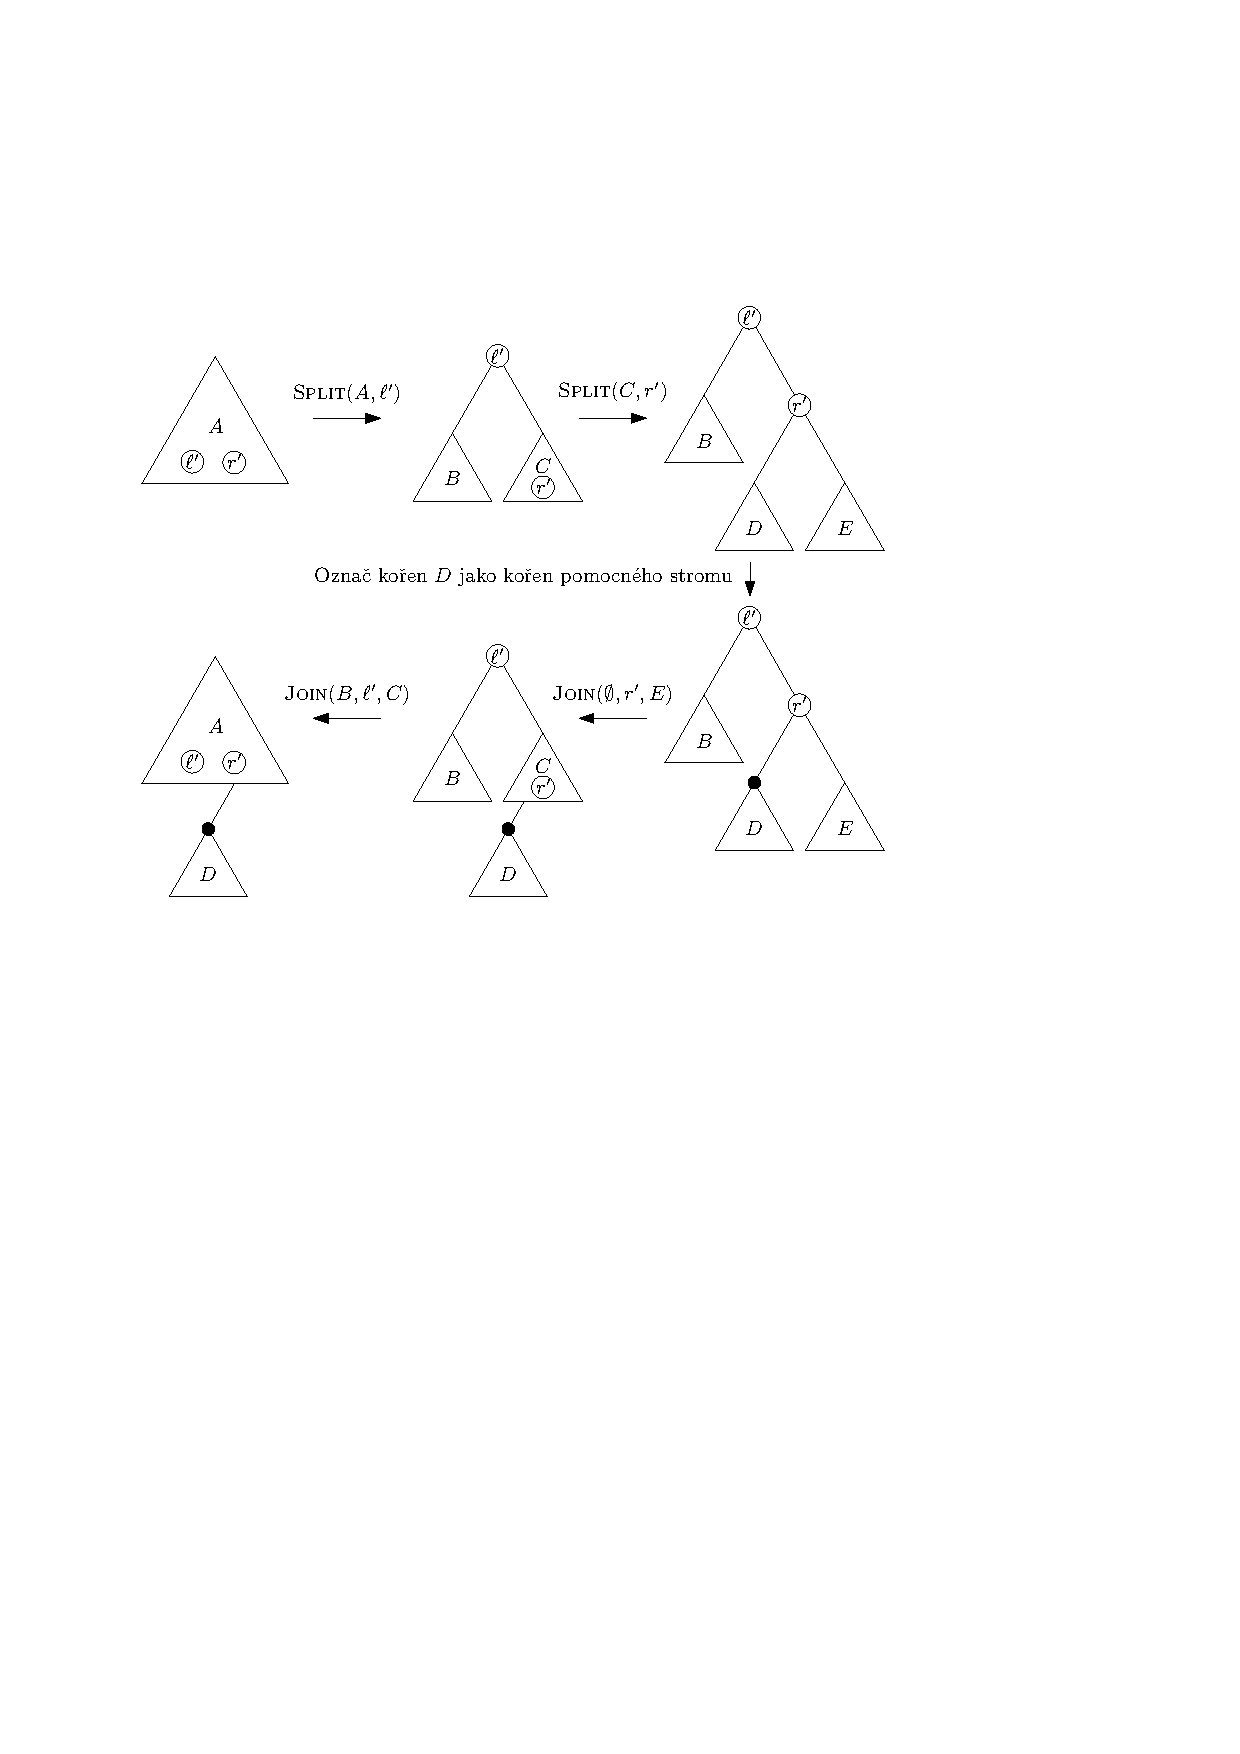
\includegraphics[width=.9\linewidth]{../img/cut_tango}
\caption{Rozdělení pomocných stromů} 

\label{obr:cut_tango} 
 
\end{figure}


Přitom vrcholy označené jako kořeny pomocných stromů považujeme za externí.
Dále najdeme předchůdce $\ell'$ vrcholu $\ell$ a následníka $r'$ vrcholu $r$. Poté zavoláme
$\ope{Split}(A, \ell')$ a dostaneme strom $B$ s~hodnotami menšími než $\ell'$,
samostatný vrchol $\ell'$ a strom $C$ s~hodnotami většími než $\ell'$. Poté
zavoláme $\ope{Split}(C,r')$ a dostaneme $D$, $r'$ a $E$. Nyní označíme kořen
$D$ za kořen pomocného stromu a připojíme ho jako levého syna vrcholu $r'$.
Dále zavoláme $\ope{Join}(\emptyset, r' E)$ a dostaneme opět strom $C$, ač
uspořádaný jinak než původně. Nakonec zavoláme $\ope{Join}(B,\ell',C)$ a
dostaneme strom $A$ s~provedenými požadovanými úpravami. V~celé operaci jsme
dvakrát hledali, dvakrát provedli \ope{Join}, dvakrát \ope{Split} a jednou
použili každou z~operací \ope{Pred} a \ope{Succ}, provedli jsme tedy $\o(1)$ operací, z~nichž každá trvá
$\o(\log |A|)\subseteq \o(\log\log n)$, celé rozdělení tedy trvalo
$\o(\log\log n)$.

Podotkneme, že operace červenočerného stromu \ope{Split} a \ope{Join} přesně tak, jak byly výše popsané, nezapadají do modelu, v němž se pohybujeme. Operaci \ope{Join} však lze v~této podobě provést pouze pomocí rotací přímočaře. U operace \ope{Split} využijeme  toho, že víme, že ovlivní pouze logaritmicky mnoho vrcholů, a víme, že libovolný strom lze převést na libovolný jiný pomocí $\o(n)$ rotací -- v tomto případě budeme postupovat, jako by část stromu, kterou \ope{Split} neovlivní, vůbec neexistovala. Připomeneme, že se v našem modelu čas strávený rozhodováním, jaký další krok máme provést, do časové složitosti nepočítá.

\section{Multisplay stromy}

\citet{multisplay} představili multisplay strom -- datovou strukturu, která se
snaží spojit dobré vlastnosti splay stromů a tango stromů. Tato struktura je
stále $(\log\log n$)-kompetitivní, ale na rozdíl od tango stromu dosahuje
amortizovaně $\o(\log n)$ na přístup (s~worst-case $\Theta(\log^2 n)$ na
přístup). Také dokáže vykonat průchod všemi prvky v~jejich pořadí v~čase
$\Theta(n)$ (na což tango strom potřebuje $\Theta(n\log\log n)$). Na rozdíl
od tango stromu bude navíc podporovat operace \ope{Insert} a \ope{Delete}\footnote{Úpravu modelu,
kterou potřebujeme k~tomu, abychom mohli mluvit o~optimalitě a kompetitivitě
struktury, která podporuje tyto operace, popíšeme později.}.

Myšlenka multisplay stromu je podobná jako myšlenka tango stromu, pouze jako
pomocné stromy nepoužívá červenočerné stromy, ale splay stromy. Vzhledem
k~tomu, že jediné operace červenočerných stromů, které tango strom využívá, jsou
\ope{Split} a \ope{Join}, lze v~tango stromech nahradit červenočerné stromy
splay stromy přímočaře, protože splay stromy tyto operace také implementují.
Samotný postup vyhledání se od tango stromu nepatrně liší. Při vyhledávání
hodnoty v~multisplay stromu nejprve najdeme odpovídající vrchol $v$ bez
jakýchkoli úprav struktury stromu a až při cestě zpět do kořene postupně
zdola nahoru měníme preferované směry vrcholů. Po změně všech preferovaných
směrů nakonec ještě změníme preferovaný směr vrcholu $v$.

Samotné měnění preferovaných směrů je v~multisplay stromu o~poznání jednodušší než v~tango stromu.
Mějme vrchol $v$ ve stromu $T$, kterému chceme změnit preferovaný směr bez újmy
na obecnost zleva doprava. Potom nám stačí nejprve zavolat \ope{Splay$(v)$}.
Následně v~levém podstromu $v$ najdeme pomocí informace o~minimální hloubce
v~podstromu daného vrcholu vrchol $\ell$, který je vrcholem s~nejvyšší hodnotou
v~tomto stromu s~hloubkou menší než $v$. Pak zavoláme \ope{Splay$(\ell)$} na levý
podstrom $v$ (tak, aby $v$ zůstal kořenem pomocného podstromu a $\ell$ se
stal jeho levým synem). Dále v~rámci pravého podstromu $v$ zavoláme \ope{Splay}
na následníka $v$. Tím se část stromu, kterou chceme z~pomocného stromu
odstranit, stala pravým podstromem levého syna kořene a pomocný strom, který
chceme nově připojit, se stal levým podstromem pravého syna kořene. Stačí tedy
upravit příznak kořene pomocného stromu v~kořenech těchto podstromů a máme
hotovo. Rozmyslíme si, že dokonce ani není potřeba upravovat hodnoty minimální
hloubky vrcholu v~podstromu kořene či jeho synů (kvůli změně příznaků; samy
předchozí operace \ope{Splay} mohou vést k~nutnosti úpravy pomocných dat).
Maximální hloubky by sice mohlo být potřeba upravit, ale ty pro algoritmus
multisplay stromu nepotřebujeme -- nebudeme je tedy ve vrcholech
udržovat.

Nyní představíme úpravy struktury, které je potřeba provést, aby bylo možné do
struktury vkládat prvky.  Pokud do multisplay stromu $T$ vložíme prvek $p$, je
nutné ho vložit i do stromu $P$. Pokud v~binárním vyhledávacím stromu vyhledáme
prvek, který v~něm není, projdeme po cestě obsahující oba jeho sousedy, přičemž
jednomu z~nich bude chybět na příslušné straně syn. To znamená, že do
multisplay stromu můžeme vložit prvek tak, že použijeme standardní algoritmus
pro vkládání do binárního vyhledávacího stromu. Vkládaný prvek nejprve označíme
za kořen (jeho vlastního jednoprvkového) pomocného stromu. Při vkládání jsme prošli
jak jeho předchůdce, tak následníka. Na hlubším z~nich musí ale vrchol $v$
s~hodnotou~$p$ viset i ve stromu $P$. Vrchol $v$ má tedy v~$P$ hloubku o~jedna vyšší,
než hlubší z~těchto dvou vrcholů. Minimální hloubky v~podstromech se tím
žádnému vrcholu (krom $v$) nezměnily, není je tedy potřeba opravovat. Nakonec
ve stromu přepneme preferované syny stejně jako při operaci \ope{Find}.

Tento postup má však jednu vadu -- všechny výše uvedené odhady časových složitostí závisí na tom, že
$P$ má hloubku $\Theta(\log n)$. Protože o~$P$ jsme dosud mluvili jako
o~nevyvažovaném stromu, mohli bychom tuto vlastnost operací \ope{Insert} rozbít.
Proto je potřeba, aby $P$ byl vyvažovaný strom. Konkrétně zvolíme červenočerný
strom, protože pro nás bude výhodné, že má amortizovaně $\o(1)$ změn barev a
worst-case $\o(1)$ rotací na operaci. V~každém vrcholu si budeme nově pamatovat
jeho barvu v~$P$ a hodnoty\footnote{Bylo by lepší, kdybychom si mohli pamatovat
přímo ukazatele na příslušné vrcholy v~$T$ (byť amortizovaná i worst-case složitost zůstane zachována). Tím bychom ale
porušili pravidla modelu, která povolují v~každém vrcholu pouze dva ukazatele,
a to na syny daného vrcholu.} jeho rodiče a synů v~$P$. 

Nyní potřebujeme umět v~$T$ provádět úpravy nutné při vyvažování $P$. To
znamená, že musíme být schopni v~$T$ najít potomka a rodiče vrcholu v~$P$ a provádět
rotaci hran. Hledání rodiče a potomka vrcholu je snadné -- rozmyslíme si, že
cesta mezi libovolným vrcholem a jeho libovolným potomkem vždy navštíví nejvýše
dva různé pomocné stromy. Protože známe hodnotu uloženou v~hledaném rodiči či
potomkovi, najdeme ho vždy pomocí nejvýše dvou operací \ope{Find} v~pomocných
stromech. Jedno nalezení potomka či následníka tedy trvá amortizovaně
$\o(\log\log n)$ (včetně změny preferovaného vrcholu, pokud příslušná cesta
vedla napříč dvěma pomocnými stromy).

Při rotaci nás čeká několik problémů. Prvním z~nich je, že musíme zachovat
invariant, že každý vrchol má právě jeden preferovaný směr. To vyřešíme změnou
preferovaných směrů. Pokud chceme například provést rotaci hrany ve vrcholu
$v$, který je v~$P$ pravým synem vrcholu $w$, musíme nastavit preferovaný směr
vrcholu~$v$ doleva a preferovaný směr vrcholu $w$ doprava. Tak dosáhneme toho,
že se při rotaci nezmění, které vrcholy náleží které preferované cestě,
může se změnit pouze jejich pořadí na ní.

Další změny struktury $P$ už se projeví pouze změnami pomocných informací
v~$T$, nikoli však změnou struktury. Tím nemáme na mysli, že bychom neprováděli
žádné rotace hran -- ještě nás čeká několik dílčích vyhledání, během nichž
provádíme v~pomocných stromech standardně operace \ope{Splay}. Již se nezmění
rozložení vrcholů mezi pomocnými stromy.

Samu rotaci pak provedeme úpravou hodnot rodičů a dětí v~dotčených vrcholech
(konkrétně je potřeba opravit vrchol, v~němž provádíme rotaci, jeho rodiče,
prarodiče a jednoho z~potomků). Dále opravíme hloubku vrcholů koncích rotované hrany. Problém ale spočívá v~tom, že nyní bychom
potřebovali opravit hloubku ve velké části stromu (například v~příkladu výše
zvýšit hloubku v~celém podstromu levého syna $\ell$ vrcholu $w$ a snížit
v~podstromu pravého syna $p$ vrcholu $v$). Všimneme si ale, že vzhledem
k~nastavení preferovaných směrů ve vrcholech $v$ a $w$ tvoří podstrom vrcholu
$\ell$ v~$P$ tytéž vrcholy jako podstrom kořene $r$ pomocného stromu
obsahujícího $\ell$ v~$T$. Podobně podstrom vrcholu $p$ v~$P$ je podstromem
kořene některého pomocného stromu v~$T$. Tyto kořeny najdeme tak, že budeme
z~kořene pomocného stromu obsahujícího $v$ a $w$ postupně hledat hodnoty
vrcholů $p$ a $\ell$, ale vždy vrátíme první vrchol s~příznakem kořene, který
najdeme (krom vrcholu, z~nějž hledat začínáme).

Nyní nahlédneme, že již dokážeme změny hloubek vyřešit v~konstantním čase pomocí některé
z~běžných technik, jako je například líná propagace změn směrem dolů, nebo, jak si
vybrali autoři multisplay stromu, diferenční kódování hloubky. To znamená, že
pouze kořen celého multisplay stromu zná svou hloubku. Ostatní vrcholy znají
rozdíl své hloubky v~$P$ a hloubky v~$P$ svého rodiče v~$T$. Stejným trikem
vyřešíme přepočítání informace o~minimální hloubce v~podstromu -- všimneme si, že
v~pomocném stromu obsahujícím $v$ a $w$ změnily hloubku pouze tyto dva vrcholy.
Proto stačí informaci přepočítat v~týchž vrcholech, jako v~případě hloubky, a
dále na cestě mezi $v$ a $w$.

Protože jsme popsali obecně, jak vykonat změnu barvy vrcholu a rotaci hrany ve
stromu, máme vše i pro implementaci operace \ope{Delete} v~multisplay
stromech\footnote{Pokud se chceme co nejpřesněji držet modelu, který jsme
zavedli, přesouvání hodnot při mazání vnitřních vrcholů tak, jak je v~binárním
vyhledávacím stromu obvyklé, není možné. Proto musíme \ope{Delete} vrcholu,
který má nějaké potomky, implementovat tak, že nejprve provedeme rotace tak,
aby se tento vrchol stal listem, až potom ho smažeme.}. Nyní bychom rádi ukázali,
že i tyto úpravy jsou staticky optimální. To je ale problematické -- náš model
nepočítal s~vkládáním a mazáním. Proto ho musíme nadefinovat znovu.

Nyní již tedy přístupová posloupnost $S$ není pouze posloupností prvků
univerza, ale posloupností operací $\ope{Find}(x)$, $\ope{Delete}(x)$ a
$\ope{Insert}(x)$, kde $x$ musí náležet univerzu. Modelu nově dovolíme dvě
nové operace, a to vložení listu na místo chybějícího syna aktuálního vrcholu,
a odstranění listu (a označení jeho rodiče za aktuální vrchol). Po každém
stromu budeme vyžadovat, aby se při vykonávání operace \ope{Find} dotkl daného
vrcholu. Dále aby při operaci \ope{Insert} navštívil (v~tomto pořadí, byť na
asymptotické chování tento požadavek nebude mít vliv) vrcholy obsahující
předchůdce a následníka vkládaného prvku a nakonec skutečně vytvořil list
s~příslušnou hodnotou. Tento požadavek je adekvátní, protože každý binární
vyhledávací strom musí oběma těmito prvky projít při vkládání. Nakonec budeme
požadovat, aby strom při operaci \ope{Delete} navštívil předchůdce mazaného
vrcholu, mazaný vrchol a nakonec následníka mazaného vrcholu. Vzhledem k~tomu,
že mazat umíme pouze listy, musíme vždy odstraňovaný vrchol rotacemi přesunout
do listu, což opět znamená, že stejně musíme předchůdce i následníka navštívit.
Tento model je již dobře nadefinovaný, proto v~něm dává smysl nadefinovat optimální strom stejně, jako v~modelu předchozím.
Pro tento model \citet{multisplay} dokázali následující větu:

\begin{veta}[Dynamic Interelave Bound]
\def\dib{\operatorname{DIB}}
Mějme referenční strom $P$. V~tomto stromu má každý vrchol svůj preferovaný
směr, buď doprava nebo doleva. Vždy, když z~vrcholu při vyhledání prvku vyrazíme
jiným než preferovaným směrem, změníme preferovaný směr tohoto vrcholu. Strom
$P$ také podporuje rotace hran a operace \ope{Delete} a \ope{Insert} (které
probíhají standardním algoritmem binárního vyhledávacího stromu\footnote{Standardní algoritmus na mazání nezapadá do nadefinovaného modelu. To
znamená, že celý náš referenční strom nesplňuje definici dynamického
binárního vyhledávacího stromu. To nevadí, strom $P$ je pomyslný a strom
$T$, který skutečně stavíme, jeho chování pouze simuluje.}). Nechť $\dib_P(S)$ je
počet změn preferovaných směrů všech vrcholů v~$P$ při vykonávání posloupnosti
operací $S$, přičemž mezi některými operacemi mohly proběhnout rotace některých
hran. Potom $$\opt(S) \in \Omega(\dib_P(S)/2 - n - 2k + cm),$$ kde $P$ je
pomocný strom včetně popisu rotací, které provádíme mezi přístupy, a~dalších
změn vzniklých vkládáním a mazáním, $n$ je počet vrcholů $P$ po poslední operaci, $k$
je počet rotací hran v~popisu $P$, $c$ je vhodně zvolená kladná konstanta a $m$
je délka posloupnosti $S$.  \end{veta}

Nahlédneme, že vzhledem k~výše uvedenému popisu mazání a vkládání je multisplay strom i v~dynamickém modelu stále $(\log\log n)$-kompetitivní. 

%\section{Geometrický náhled na stromové operace}
